\documentclass[hidelinks, 12pt]{article}
\usepackage[utf8]{inputenc}
\def\magyarOptions{defaults=hu-min}
\usepackage[english,magyar]{babel}
\usepackage{t1enc}
\hyphenation{huhyphc}
\usepackage[document]{ragged2e}
\usepackage{geometry, array, graphicx, wrapfig, float, amsmath, titlesec, amsmath, amsfonts, mathtools, amssymb, colortbl, babel, listings, hyperref, caption, textcomp, eurosym}
\usepackage[thinlines]{easytable}
\graphicspath{ {./pics/} }
\geometry{a4paper, inner=3.5cm, outer=2.5cm, bottom=2.5cm, top=2.5cm}
\renewcommand{\baselinestretch}{1.5}
\renewcommand{\arraystretch}{0.8}
\setlength{\parskip}{1em}
\makeatletter
\makeatother
\frenchspacing
\begin{document}
	\makeatletter
	\renewcommand*{\thetable}{\arabic{table}}
	\renewcommand*{\thefigure}{\arabic{figure}}
	\let\c@table\c@figure
	\makeatother
	\captionsetup[figure]{name=Ábra}
	\captionsetup[table]{name=Ábra}
	\newcommand{\sectionbreak}{\clearpage}
	\begin{titlepage}
		\begin{minipage}{0.36\textwidth}
			\begin{figure}[H]
				\includegraphics[scale=0.1]{elte_cimer_szines.jpg}
			\end{figure}
		\end{minipage}
		\begin{minipage}{0.60\textwidth}
			\begin{center}
				{\Large Eötvös Loránd Tudományegyetem \\
					Informatikai Kar \\
					Komputeralgebra Tanszék \\}
			\end{center}
		\end{minipage}
		\\[0.3\baselineskip]
		\noindent\makebox[\linewidth]{\rule{\textwidth}{0.5pt}}
		\vspace*{\fill}
		\centering
		\vspace*{0.5cm}
		
		\huge\bfseries
		Pszeudovéletlen sorozatok mértékei és konstrukciói		
		\vspace*{0.5cm}
		
		\vspace*{\fill}
		\begin{TAB}(r,0.5cm,0.5cm)[9pt]{cc}{cccc}
			\normalfont \normalsize \textsl{ Szerző: } & \normalfont \normalsize \textsl{ Témavezető: } \\
			\normalsize Kovács Levente & \normalsize Dr. Tóth Viktória \\
			\normalfont \normalsize programtervező informatikus BSc & \normalfont \normalsize egyetemi adjunktus \\
			\normalsize & \normalfont \normalsize Komputeralgebra Tanszék
		\end{TAB}
		\\
		\large \normalfont Budapest, 2019
	\end{titlepage}
	\renewcommand*\contentsname{Tartalomjegyzék}
	\tableofcontents
	\newpage
	\section{Bevezető}
	\subsection{Történeti betekintés}
	Véletlen sorozatok generálására sok modern területnek igénye van (pl.: statisztika, szimulációk, kriptográfia). Algoritmikusan azonban nem lehetséges valódi véletlen számokat generálni, ezért pszeudovéletlen eljárásokra hagyatkozunk. Cél az, hogy olyan eljárásokat használjunk, melyek eredményei statisztikailag véletlennek tűnnek, attól függetlenül, hogy egy determinisztikus rendszer generálja az eredményt.
	\par
	Az ilyen sorozatokra való igény először Gilbert Vernam munkájának következménye. 1917-ben Vernam feltalálta a one-time pad titkosítási eljárást. Az üzeneteket telegráfon bitenként továbbították, viszont az eredeti adatot valamilyen kulcs segítségével megváltoztatták (amit aztán a fogadó fél a kulcs ismeretében vissza tud fejteni). Ha le is hallgatták a küldött adatot, akkor a kulcs nélkül nem lehetett tudni, hogy mi volt az eredeti üzenet.
	\par
	1949-ben Claude Shannon, matematikus, bebizonyította a fenti eljárásról, hogy ha egy jó sorozatot használunk kulcsnak, akkor az eredeti és a titkosított bitsorozat között nem lehet semmiféle összefüggést találni \cite{shannon}. Ennek következménye, hogy a Vernam-féle one-time pad eljárást nem lehet feltörni, ha megfelelő, egyszer használatos kulcsokat használunk.
	\par
	Az is igaz azonban, hogy ha nem megfelelően választjuk meg a kulcsokat (pl. többször használunk egy titkosító kulcsot), akkor a titkosítás könnyen törhető. A fő nehézség tehát a one-time pad használatánál, hogy nagy méretű véletlen bitsorozatokat kell előállítani kulcsoknak.
	\par
	Az ilyen sorozatok előállításához régen fizikai eszközöket használtak, pl. diódákat. A problémája az ilyen eszközöknek, hogy külső tényezők is befolyásolják a véletlenséget, és meghibásodás is történhet. Ezért nagyon fontos a véletlenség vizsgálása különböző statisztikai tesztekkel, ami azonban időigényes. Emiatt jobb, hogy ha "csak" pszeudovéletlen sorozatokat állítunk elő. Így elkerülhető a statisztikai tesztelés, mivel bizonyítottan jó véletlen tulajdonságokkal rendelkező sorozatot kapunk.
	\par
	A pszeudovéletlen tulajdonságok mérésével sok évtizede foglalkoznak matematikusok. Elsőként Émile Borel definiálta végtelen bináris sorozatokra a pszeudovéletlenség normalitás mértékét \cite{borel}. Később Solomon Wolf Golomb és Donald Knuth \cite{knuth} próbálkoztak a pszeudovéletlenség matematikai fogalmának definiálásával. Ennek a definíciónak alapvető gyengeségei voltak, ezért ezt ma már nem nagyon használják. Ezután Andrej Nyikolajevics Kolmogorov \cite{kolmogorov} és Gregory John Chaitin bonyolultságelméleti irányból közelítették meg a problémát, de a gyakorlatban ezek a fogalmak nem kaptak nagy jelentőséget, mivel alkalmazásuk nem jól kivitelezhető.
	\par
	Ezen próbálkozások inspiráltak egy új, konstruktív megközelítést a pszeudovéletlenség vizsgálatára. Christian Manduit és Sárközy András megközelítése az volt, hogy léteznek olyan sorozatok, melyekről bizonyítható, hogy statisztikailag erős véletlen tulajdonságokkal rendelkeznek (más szóval: erős pszeudovéletlen tulajdonságúak), így az utólagos tesztelés elkerülhető. Ez a fajta vizsgálat az évek során egyre szélesebb körben alkalmazott. \cite{sarkozymauduit}
	\subsection{A program célja}
	A programom célja, hogy a fent említett konstrukció keretén belül vizsgáljak különböző pszeudovéletlen generátorokat. A vizsgált konstrukciókat két csoportból válogattam. Egyik kategóriába matematikai hátterű sorozatok tartoznak, melyeknek működése főként számelméleti ismereteken alapulnak. A másik csoport az iparban széles körben használt pszeudovéletlen generátorok, amik nem feltétlenül matematikai hátterűek.
	\par
	A programban lehetőség nyílik a pszeudovéletlen konstrukciók kipróbálására, és a generált sorozatok vizsgálatára a statisztikai mértékek szerint. A sorozatokat ki is próbálhatjuk a Vernam-féle one-time pad titkosítási eljárással.
	\newpage
	\section{Felhasználói dokumentáció}
	A program pszeudovéletlen sorozatkonstrukciók kipróbálására és a sorozatok vizsgálatára készült statisztikai mértékekkel.
	\subsection{Rendszerkövetelmények}
	A telepítéshez szükséges a rendszeren a TDM-GCC fordító és a make megléte. A TDM-GCC a \url{https://sourceforge.net/projects/tdm-gcc/} oldalról ingyenesen elérhető, a make pedig Windows esetén a \url{http://gnuwin32.sourceforge.net/packages/make.htm} oldalon érhető el, Linux rendszeren terminálból telepíthető. Ha nem történt volna meg, ezeknek az útvonalát adjuk hozzá a PATH környezeti változóhoz.
		
	Szükséges egy telepített és megfelelően konfigurált QT5 keretrendszer mingw73\_64-es platformra. Ez is ingyenesen telepíthető a \url{https://www.qt.io/download} oldalról.
	
	A megfelelően konfiguráltság annyit jelent, hogy könyvtárak és a qmake utai hozzá kell legyenek adva a rendszer PATH környezeti változójához, hogy a program megtalálja a megfelelő .dll fájlokat. Jelen esetben a $<$QT helye$>$ mingw73\_64\textbackslash bin mappát kell hozzáadni a PATH-hoz (a qmake és a .dll-ek egy mappába vannak).
	\subsection{Telepítés}
	Ha a fenti függőségek megfelelően telepítve vannak, akkor telepíthető a program. A Setup mappában található setup.bat script lefuttatja a qmake-et és a make-et, ezzel a program fájljait fordítva és létrehozva a futtatható állományt.
	\subsection{Futattás}
	Ha a QT megfelelően van konfigurálva, akkor a Setup release mappájában lévő pszeudoveletlen\_szakdolgozat.exe fájl futtatásával lehet elindítani a programot.
	\subsection{Menürendszer}
	A menürendszer pontjainak 3 fő csoportja van, ezek:
	\begin{itemize}
		\item Alapvető funkciók: Kilépés, vissza a főmenübe
		\item Konstrukciók: A konstrukciók kipróbálása
		\item Tesztelés: Mértékek és titkosítás
	\end{itemize}
	\subsubsection{Főmenü}
	Amikor a program elindul, a felhasználót a főmenü fogadja. Itt elérhető az összes megvalósított konstrukció almenüpontja és a mértékek, illetve titkosításé is.
	
	\begin{figure}[h]
		\centering
		\begin{minipage}{\textwidth}
			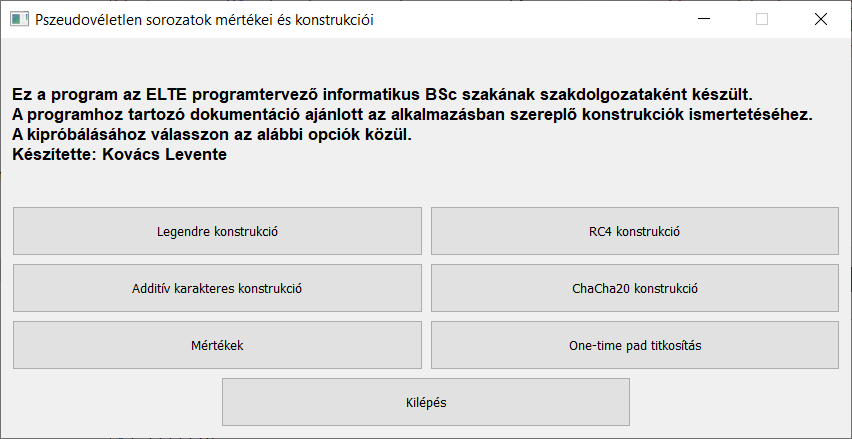
\includegraphics[width=\textwidth]{mainmenu.png}
		\end{minipage}
		\caption{Főmenü}
	\end{figure}
	
	Kilépni a program jobb felső sarkában található "X" gombbal, vagy a főmenüben lévő "Kilépés" gombbal lehet.

	\subsection*{Konstrukciók}
	Ez a pont csak alapvető segítséget nyújt a különböző konstrukciók kipróbálásához. Részletes leírása az algoritmusoknak a fejlesztői dokumentációban találhatóak.
	\par
	\subsubsection{Legendre szimbólumos konstrukció}
		Ez a konstrukció a Legendre szimbólumon alapul, melynek véletlen tulajdonságait régóta vizsgálják. Mauduit és Sárközy ezen a sorozaton vizsgálta először 1997-ben a véges bináris sorozatokra készített jól-eloszlás és korreláció-mértékeket. \cite{sarkozymauduit}
	\par
	Szükséges paraméterek:
	\begin{enumerate}\bfseries
		\item A sorozat hossza
		\\ \normalfont{A sorozat hosszát bitekben kell megadni. Bármennyi lehet.}
		\bfseries \item Prímszám
		\\ \normalfont Egy olyan prímszámra van szükségünk a konstrukcióhoz, mely legalább 16-szor nagyobb mint a sorozat hossza (bitben megadott méret esetén 2-szer nagyobb). Az is kell, hogy a 2 legyen primitív gyök modulo prím. A "Generálás" gombbal a program megkeresi a legkisebb olyan prímet, mely a fenti feltételeknek megfelel. A "Következő" gombbal ugorhatunk a következő jó prímre.
		\bfseries \item A konstrukcióhoz használt polinom fokszáma \\ \normalfont
		A fokszám nem lehet túl nagy függően a prímszámtól, de túl kicsi sem. Az alsó határ jelen megvalósításban 2-nek, a felső $5\cdot\sqrt[\leftroot{-2}\uproot{2}10]{p}$-nek lett megszabva, ahol $p$ a használt prímszám. Polinom fokszámot generálhatunk a fenti intervallumban a "Generálás" gombbal.
		\bfseries \item A polinom \\
		\normalfont
		A konstrukció jó működéséhez szükséges, hogy olyan polinomot válasszunk, amelynek csak egyszeres gyökei vannak. Emiatt a polinomot a gyökeinek felsorolásával reprezentáljuk, ezeket szóközzel elválasztva kell felsorolni a szövegmezőben. A fokszámmal megegyező számú gyököt kell megadni. Lehetőség van polinom generálására is, ekkor a program legenerál egy az előző pontban megadott fokszámú polinomot.
	\end{enumerate}
	
	\begin{figure}[h]
		\centering
		\begin{minipage}{\textwidth} % choose width suitably
			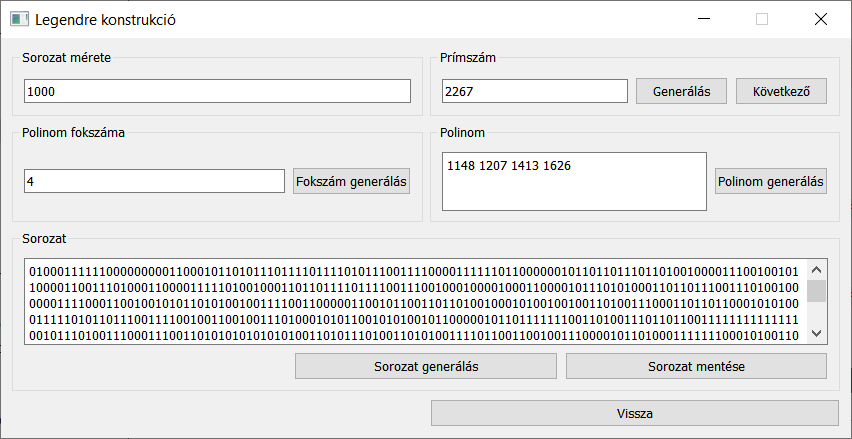
\includegraphics[width=\textwidth]{legendremenu.png}
		\end{minipage}
		\caption{Legendre menü}
	\end{figure}
	Ha a fenti paramétereket megadtuk, akkor a "Sorozat generálása" gombra kattintva megkapjuk az eredményét a Legendre konstrukciónak a kapott bemenetre.
	\subsubsection{RC4 konstrukció}
	Az RC4 konstrukciót Ron Rivest fejlesztette ki 1987-ben, viszont eredetileg üzleti titok volt. 1994-ben azonban kiszivárgott az algoritmus leírása. \cite{rcleak} A működése egyszerű és gyors, ezért használata széles körben elterjedt, viszont vannak rossz tulajdonságai.
	\par
	Szükséges paraméterek:
	\begin{enumerate}
		\bfseries\item A sorozat hossza \\
		\normalfont A sorozat hosszát bitekben kell megadni. Bármennyi lehet.
		\bfseries \item A kulcs
		\\
		\normalfont A kulcs változó méretű lehet, ez alapján fog történni a generálás. Tipikusan 40-2048 bit hosszú a kulcs. Ez a megvalósítás egy szöveget vár kulcsnak, így átfogalmazva a feltételt legalább 5, maximum 256 karakter hosszú lehet a kulcs.
	\end{enumerate}
	\begin{figure}[h]
		\centering
		\begin{minipage}{\textwidth} % choose width suitably
			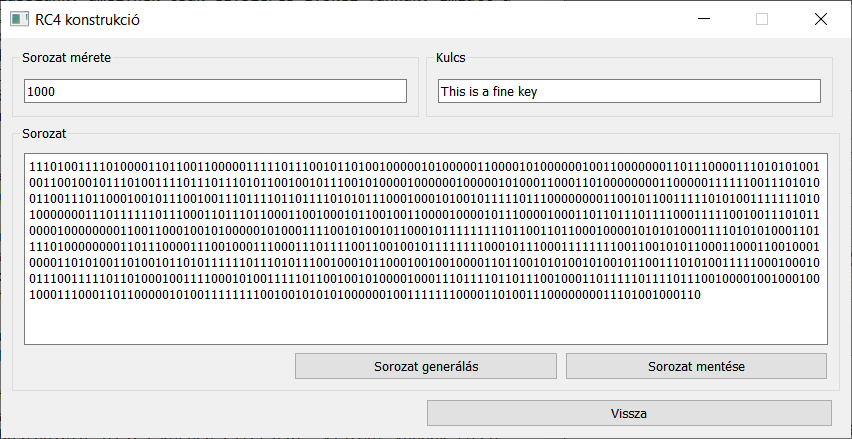
\includegraphics[width=\textwidth]{RC4menu.png}
		\end{minipage}
		\caption{RC4 menü}
	\end{figure}
	A fenti paraméterek megadása után megtekinthetjük az RC4 konstrukció által generált sorozatot a "Sorozat generálása" gombbal.
	\subsubsection{Additív karakteres konstrukció}
	Ezt a konstrukciót Mauduit, Rivat és Sárközy vezették be. \cite{additive} \par
	Szükséges paraméterek:
	\begin{enumerate}
		\bfseries \item A sorozat hossza \\
		\normalfont A sorozat hosszát bitekben kell megadni. Bármennyi lehet. \\
		\bfseries \item Prímszám \\
		\normalfont Ebben a konstrukcióban a prímszám nagyságára nincs igazi nagyságrendi követelmény. A "Generálás" gombbal a legkisebb, sorozat hosszánál nagyobb prímszámot adja vissza. A "Következő" gomb megkeresi az első jelenleginél nagyobb prímet.
		\bfseries \item A konstrukcióhoz használt polinom fokszáma \\
		\normalfont Hasonlóan a Legendre konstrukcióhoz, a fokszámtól elvárjuk, hogy ne legyen túl nagy vagy túl kicsi. Az alsó határ jelen megvalósításban 2-nek, a felső $5\cdot\sqrt[\leftroot{-2}\uproot{2}10]{p}$-nek lett megszabva, ahol p a használt prímszám. A "Generálás" gombbal egy fokszámot kapunk a fenti intervallumból.
		\bfseries \item A polinom \\
		\normalfont A Legendre konstrukcióhoz hasonlóan fontos, hogy a polinomnak csak egyszeres gyökei legyenek. Ezért a polinomot legenerálhatjuk úgy, hogy a gyökeit soroljuk fel, szóközzel elválasztva. A fokszámmal megegyező számú gyököt kell megadni. Lehetőség van polinomot generálni a fenti követelményeknek eleget téve a "Polinom generálása" gombbal.
	\end{enumerate}
	A fenti paraméterek megadása után megtekinthetjük az additív karakteres konstrukció által generált sorozatot a "Sorozat generálása" gombbal.
	\begin{figure}[h]
		\centering
		\begin{minipage}{\textwidth} % choose width suitably
			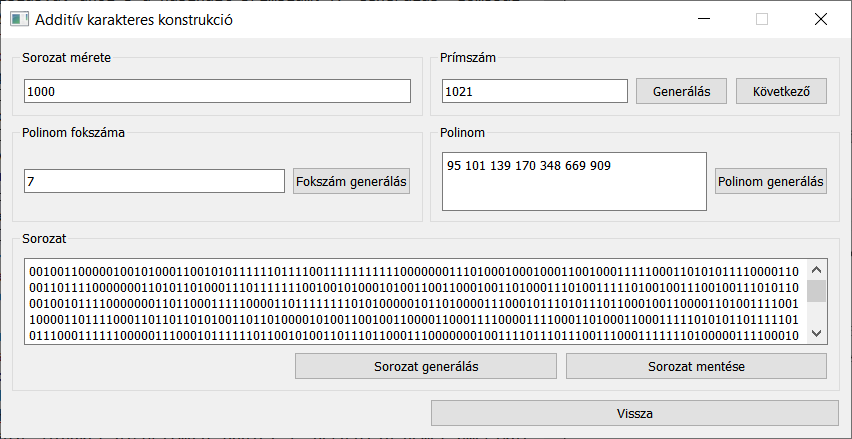
\includegraphics[width=\textwidth]{additivemenu.png}
		\end{minipage}
		\caption{Additív karakter menü}
	\end{figure}
	\subsubsection{ChaCha20 konstrukció}
	A ChaCha20 egy stream cipher eljárás, mely a Salsa20 egy változata. Mindkét algoritmust Daniel J. Bernstein német-amerikai matematikus, kriptológus fejlesztette ki. A Salsa változatot 2005-ben tervezte, 2007-ben publikálták először \cite{salsa}, az eSTREAM projekt keretében. A ChaCha változat 1 évvel később, 2008-ban lett publikálva, célja az volt, hogy növelje a lavinahatást és ugyanolyan, vagy picit jobb teljesítményű legyen, mint a Salsa. \cite{chacha}
	
	Mindkét eljárás eszközei a bitenkénti XOR (kizáró vagy), a 32-bites összeadás $\textrm{mod}\ 2^{32}$, és a konstans távolságú forgatás egy belső állapoton, ahol az állapot 16 db 32-bites adatból (szóból) áll. Csak ezen műveletekkel az algoritmus kivédi az időzítéses támadásokat. Ez olyan támadás, ahol a támadó fél a futtató rendszer hiányosságait kihasználva (tehát nem a szoftver implementációja a baj) a kriptográfiai algoritmus futási idejéből próbálja feltörni a rendszert, mivel a bemenettől függhet a futási idő. Csak fix 32-bites műveleteket használva a futási idő megegyezik minden bemenetre, mivel az algoritmus fixen 20 menetben végzi el a fenti műveleteket és a műveletek száma is fix minden menetben.
	
	A ChaCha algoritmus állapotrendszerének és algoritmusa részletes leírása a fejlesztői dokumentációban található. Jelen megvalósítás az RFC 8439-ben \cite{RFC} definiáltakat követi, melyet az IRTF publikált 2018-ban, de ezen kívül több változata van az algoritmusnak, főként a körök számára vonatkozóan.
	
	A szükséges bemenetek:
	\begin{enumerate}
		\bfseries \item A sorozat hossza \\
		\normalfont A sorozat hosszát bitekben kell megadni. Bármennyi lehet.
		\bfseries \item Kezdőállapot \\
		\normalfont A kezdőállapot 16 darab 32 bites szóból áll, jelen implementációban az egyszerűbb használat miatt 16 darab előjel nélküli 32 bites egész számot jelent. Az állapot 4 részre bomlik, ebből az egyik kategória konstans, 4 darab szóval, így ezt nem kell megadni. A maradék 3 csoport 12 szavát kategóriánként kell megadni:
		\begin{enumerate}
			{\itshape \item {Kulcs}} \\
			Ez 8 darab állapotot fed le. Jelen esetben 8 darab számot kell megadni a $[0, 2^{32}-1]$ intervallumban. Tudunk kulcsot generálni a fenti intervallumból vett számokkal a "Generálás" gombra kattintva.
			{\itshape \item {Számláló}} \\
			A jelen megvalósításban ez egy szót fed le (van verzió, ahol 64 bites a számláló, vagyis 2 szót foglal le), a megvalósításban ez minden "körében" az algoritmusnak növelődik, mondhatni számolja az iterációkat. Egy számot kell megadni a $[0, 2^{32}-1]$ intervallumban.
			{\itshape \item {Egyszer használatos kulcs (nonce)}} \\ 
			Ez a maradék 3 szót foglalja magában. Ez a kulcs azért van külön kategóriában, mert ezt a kulcsot csak egyszer lehet használni egy titkosított kommunikációban, hogy kivédje az újraküldéses támadásokat. Ez általában egy tetszőleges szám, de mindig más. Jelen megvalósításban ez 3 darab szám megadása a $[0,2^{32}-1]$ intervallumban. Generálhatunk ilyen egyszer használatos kulcsot a fenti intervallumból vett számokkal a "Generálás" gombra kattintva.
		\end{enumerate}
	\end{enumerate}
	A fenti paraméterek megadása után megtekinthetjük az ChaCha20 konstrukció által generált sorozatot a "Sorozat generálása" gombbal.
	\begin{figure}[h]
		\centering
		\begin{minipage}{\textwidth} % choose width suitably
			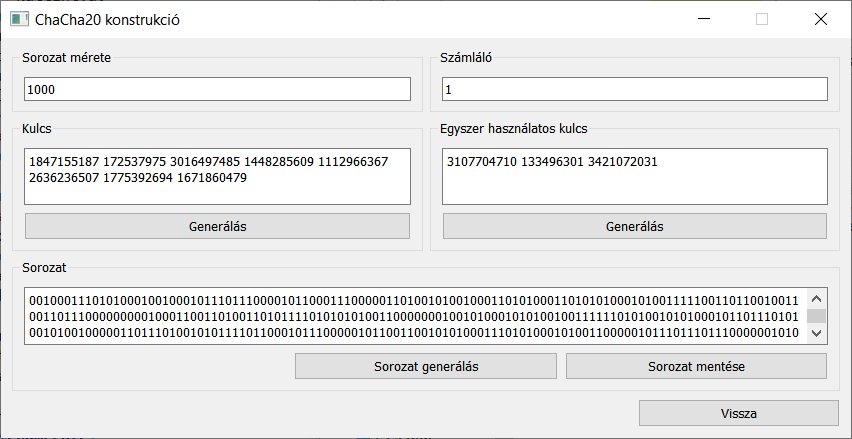
\includegraphics[width=\textwidth]{chachamenu.png}
		\end{minipage}
		\caption{ChaCha20 menü}
	\end{figure}
	\subsection{Mértékek}
	Ezen része a programnak az átlagos felhasználónak nem feltétlenül tud sokat nyújtani. Ahhoz, hogy a mértékek eredményeit értelmezni tudjuk, szükséges a formulákról és a jelentésükről való ismeret megszerzése. Ezen ismeretek alapjait a fejlesztői dokumentációban részletezem, a dokumentáció ezen részén csak röviden foglalom össze a program funkcióit.
	
	Három fő mértékünk van:
	\begin{enumerate}
		\bfseries \item Jól-eloszlás
		\bfseries \item Normalitás 
		\bfseries \item Korreláció
	\end{enumerate}
	Ezekből kettőt közvetlenül ki tudunk számolni, de a harmadikra csak közelítő értéket ad a program, mivel a számolás műveletigénye olyan nagyságrendeket ér el, hogy ennek kivárása rengeteg időbe telne a szakdolgozat keretein belül.
	
	A számolási paraméterek:
	\begin{enumerate}
		\bfseries \item A vizsgálandó sorozat \\
		\normalfont A sorozat, melyre ki szeretnénk számolni a mértékeket. Korábban mentett sorozat betölthető a "Sorozat betöltése" gombbal, de saját magunk is írhatunk be tetszőleges sorozatot. \\
		A jól-eloszlás és a normalitás mértékek számolásához további paraméter nem szükséges, ezeket kiszámolhatjuk a "Számolás" gombbal. \\
		\bfseries \item A k-ad rendű korreláció közelítésének rendje és menetszáma \\
		\normalfont Ennek a mértéknek a számolása, mint fent említettem, túlságosan nagy műveletigényű a dolgozat keretein belül, ezért csak közelítő eredményt adunk a k-ad rendű korrelációra (gyakorlatilag ezeknek a maximuma a korreláció mérték). Meg kell adnunk, hogy hányad rendű korrelációt szeretnénk vizsgálni, és hogy hány menetes a számolás (hányszor próbálkozik új sorozattal). Hasonlóan a többi mértékhez, a "Számolás" gombbal tudjuk elkezdeni a műveletet.
	\end{enumerate}
	\begin{figure}[h]
		\centering
		\begin{minipage}{\textwidth} % choose width suitably
			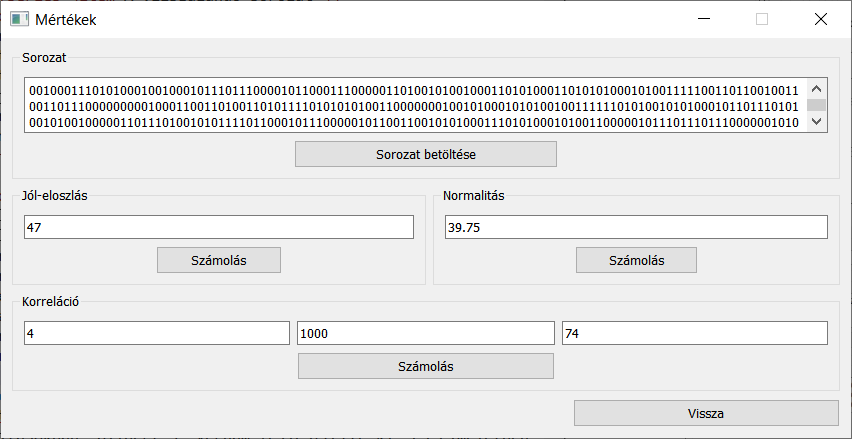
\includegraphics[width=\textwidth]{measuremenu.png}
		\end{minipage}
		\caption{Mértékek menü}
	\end{figure}
	\subsection{One-time pad titkosítás}
	A One-time pad eljárásnak széleskörű alkalmazásai vannak a titkosításokban. Gilbert S. Vernam fejlesztette ki, és elméletben tökéletes titkosságot nyújt megfelelően véletlen bemenő paraméter esetén. \cite{shannon}
	
	Használatához először egy titkosítandó szöveget kell megadni, mely a magyar billentyűzet legtöbb betűjét tartalmazza. Kivételek a ritkán használt szimbólumkarakterek mint pl. a '˙', teljes listát a fejlesztői dokumentáció tartalmazza. A titkosításhoz használt bitsorozatot kell még megadni, mely fontos, hogy legalább olyan hosszú legyen, mint a bemenő szöveg karaktereinek számának 7-szerese. Eredményként a titkosított szöveget kapjuk a fenti karakteres formában.
	
	Bemenő paraméterek:
	\begin{enumerate}
		\bfseries \item Titkosítandó szöveg \\
		\normalfont A szöveget amit titkosítani szeretnénk, a magyar billentyűzet legtöbb karakterét tartalmazhatja. Hosszúsága bármennyi lehet.
		\bfseries \item Titkosító bitsorozat \\
		\normalfont A bitsorozat, mely a titkosítás kulcsaként szolgál. Betölthető korábban lementett sorozat a "Sorozat betöltése" gombbal, de magunk is írhatunk be sorozatot. Fontos, hogy a bitsorozat hossza legalább annyi legyen, mint a titkosítandó szöveg karakterszámának 7-szerese. A titkosítást különben nem lehet elvégezni. \\
		Ezután a "Szöveg titkosítása" gombra kattintva lefuttathatjuk a titkosítást és megtekinthetjük az eredményt a "A titkosított szöveg" fülnél. Ezt a szöveget visszafejthetjük az eredetivé, ha az eredeti kulcsként használt bitsorozattal újra lefuttatjuk a titkosítást a titkosított szövegen.
	\end{enumerate}
	\begin{figure}[h]
		\centering
		\begin{minipage}{\textwidth} % choose width suitably
			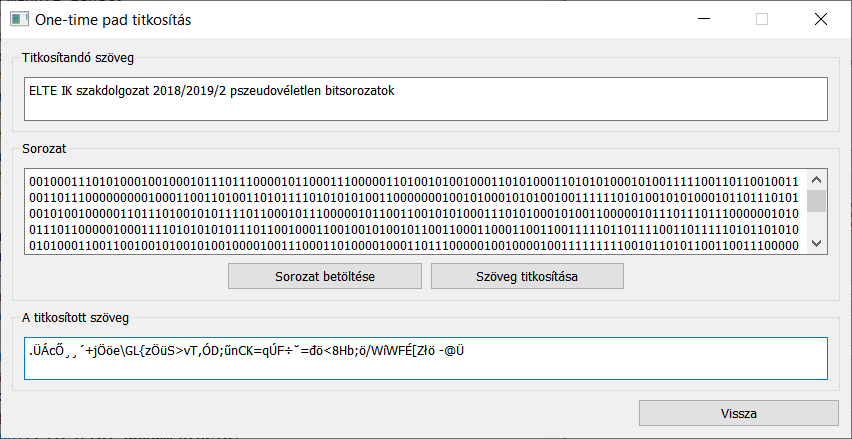
\includegraphics[width=\textwidth]{onetimepadmenu.png}
		\end{minipage}
		\caption{One-time pad titkosítás menü}
	\end{figure}
	\newpage
	\section{Fejlesztői dokumentáció}
	\subsection{Konstrukciók}
	\subsubsection{Legendre konstrukció}
	\subsubsection*{Ismertető}
	\textbf{Def.}: Ha $p$ egy prímszám, és $a \in \mathbb{Z}$, akkor az $\left({\frac{a}{p}}\right)$ Legendre-szimbólum értéke: \par
	$$\left({\frac{a}{p}}\right) =
	\begin{cases*}
	1 & ha $a$ kvadratikus maradék modulo $p$ és $a \not\equiv 0\ (\textrm{mod}\ p)$ \\
	-1       & ha $a$ nem kvadratikus maradék modulo $p$\\
	0 & ha $a \equiv 0\ (\textrm{mod}\ p)$
	\end{cases*}$$
	A Legendre-szimbólum véletlenségét már régóta vizsgálták, ez volt a motiváció a konstrukció megvalósítására.
	\subsubsection*{Algoritmus}
	\begin{enumerate}
		\item Vegyünk egy olyan $p$ prímet, hogy a $2$ legyen primitív gyök modulo $p$
		\item Vegyünk egy olyan $f \in \mathbb{F}_p[x]$ polinomot, melynek csak egyszeres gyökei vannak, és foka nem túl nagy p-hez képest
		\item $k$ hosszú sorozat esetén a ($e_0, e_1, ..., e_{k-1}$) sorozat $i$. tagja: $$e_i = 
		\begin{cases*}
		 \left({\frac{f(i)}{p}}\right) &, ha $p \nmid f(i)$  \\
		1 &, ha $p \mid f(i)$ 
		\end{cases*}
		$$
	\end{enumerate}
	\subsubsection*{Extra követelmények}
	Ha egy $n$ hosszú sorozatot szeretnénk generálni, akkor a használt $p$ prímre legyen igaz, hogy $p > 2n$. A polinom fokszáma szeretnénk, ha nem lenne túl kicsi, és a felső határt $p$-hez viszonyítva kell megadni. Jelen megvalósításban ha $k$ a polinom fokszáma, akkor legyen $2 \leq k \leq 5\cdot\sqrt[\leftroot{-2}\uproot{2}10]{p}$.
	\subsubsection{RC4 konstrukció}
	\subsubsection*{Ismertető}
	Az RC4 stream cipher algoritmus a bájt hosszúságú bitsorozatok egy permutációjának előállításával kezdődik, ami egy kulcssorozat segítségével történik. Ez a key-scheduling fázisa az algoritmusnak.
	\par
	Ez után következik a tényleges sorozat generálás. Ameddig kell a sorozatot generálni (pl. hossz alapján), addig az algoritmus lépésenként keveri a bájtok sorrendjét, és közben egy bájtnyi kimenetet generál.
	\par
	Ebben a megvalósításban a klasszikus, módosítások nélküli algoritmust valósítottam meg, hogy ez hogyan viszonyul a megvalósított mértékekhez.
	A módszernek több változata van, amik javíthatják a véletlenségét a generált sorozatnak.
	\subsubsection*{Algoritmus}
	\begin{enumerate}
		\item Töltsünk fel egy 256 elemű $S$ tömböt úgy, hogy $i$. indexére: $S[i]:=i$. 0-tól indexelünk, és gyakorlatilag az összes 8 hosszúságú bitsorozatot kell előállítani
		\item Adjunk meg egy $n$ méretű $K$ (ebben a megvalósításban egy $n$ karakterű ASCII kódolású szöveg) kulcstömböt, ahol $1 \leq n \leq 256$
		\item Ez az algoritmus key-scheduling fázisa. Legyen $i, j:=0$, majd:
			\begin{enumerate}
				\item Legyen $j:=(j+S[i]+K[i \ \textrm{mod}\ n]) \ \textrm{mod} \ 256$
				\item Cseréljük ki $S[i]$ és $S[j]$ értékét
				\item Inkrementáljuk $i$-t, ha $i < 256$, akkor ugorjunk vissza (a)-ra
			\end{enumerate}
		\item Ez a sorozatgeneráló fázis. Legyen $i, j := 0$, $n$-szer kell generálni 1 bájtnyi kimenetet, tehát ennek követésére legyen $l:=0$, majd:
		\begin{enumerate}
			\item Legyen: $i := (i+1) \ \textrm{mod} \ 256$, majd $j := (j + S[i]) \ \textrm{mod} \ 256$
			\item Cseréljük ki $S[i]$ és $S[j]$ értékét
			\item Legyen $T := S[(S[i] + S[j]) \ \textrm{mod} \ 256]$, T lesz a mostani generálási lépés 1 bájtnyi kimenete
			\item Inkrementáljuk $l$-t, ha $l < n$, akkor ugorjunk vissza (a)-ra
		\end{enumerate}
	\end{enumerate}
	\subsubsection*{Extra követelmények}
	Elvárjuk, hogy a kulcssorozat ne legyen túl rövid (általában 40 bit az alsó határ). Jelen megvalósításban: $n \geq 5$, vagyis legalább 5 karakter hosszú kulcs kell.
	\subsubsection{Additív karakteres konstrukció}
	\subsubsection*{Bevezető}
	Az additív karakteres konstrukció a Legendre szimbólumoshoz áll legközelebb. A Legendre szimbólumos konstrukció jobb véletlenségi tulajdonságokat mutat. Az additív karakteres sorozat azonban nagyobb sorozatcsaládot képes előállítani, és implementációja egyszerűbb.
	
	Nevét a konstrukció jó tulajdonságait bizonyító tételben használt additív karakterekről kapta.
	\subsubsection*{Algoritmus}
	\begin{enumerate}
		\item Vegyünk egy páratlan $p$ prímet
		\item Vegyünk egy olyan $f \in \mathbb{F}_p[x]$ polinomot, melynek csak egyszeres gyökei vannak, és foka nem túl nagy $p$-hez képest
		\item $k$ hosszú sorozat esetén a ($e_0, e_1, ..., e_{k-1}$) sorozat $i$. tagja: $$e_i = 
		\begin{cases*}
		1 &, ha $f(i) \ \textrm{mod} \ p  < \frac{p}{2}$  \\
		0 &, ha $\frac{p}{2} \leq f(i) \ \textrm{mod} \ p$ 
		\end{cases*}
		$$
	\end{enumerate}
	\subsubsection*{Extra követelmények}
	A polinom fokszáma szeretnénk, ha nem lenne túl kicsi, és a felső határt $p$-hez viszonyítva kell megadni. Jelen megvalósításban ha $k$ a polinom fokszáma, akkor legyen $2 \leq k \leq 5\cdot\sqrt[\leftroot{-2}\uproot{2}10]{p}$.
	\subsubsection{ChaCha20 konstrukció}
	\subsubsection*{Bevezető}
	A ChaCha20 stream cipher eljárás egy belső állapoton végzett bitenkénti XOR (kizáró vagy), összeadás ($ \textrm{mod} \ 2^{32}$) és konstans távolságú forgatásokkal működik. Az állapot 16 darab 32 bites szóból tevődik össze, melynek kezdeti felépítése:
	
	\begin{table}[h]
	\centering
		\begin{tabular}{|c|c|c|c|}
			\hline
			\rowcolor{yellow}Const&Const&Const&Const\\\hline
			\rowcolor[rgb]{0.04313,0.7137,1} Key&Key&Key&Key\\\hline
			\rowcolor[rgb]{0.04313,0.7137,1} Key&Key&Key&Key\\\hline
			\cellcolor[rgb]{1,0.3686,0.3686}Counter& \cellcolor[rgb]{0,1, 0.26}Nonce&\cellcolor[rgb]{0,1, 0.26}Nonce&\cellcolor[rgb]{0,1, 0.26}Nonce\\\hline
		\end{tabular}
	\caption{ChaCha20 állapot szerkezete}
	\end{table}
	A konstans mezők együttes értéke az "expand 32-byte k" szöveget adja ki. A fő művelet az úgynevezett negyedkör (quarter round), ez egy 4 paraméteres eljárás, melynek minden paramétere egy 32-bites szó változója. Jelöljük ezt QR($a$, $b$, $c$, $d$)-vel, ekkor a QR($a$, $b$, $c$, $d$) eljárás (C stílusú pszeudokódként):
	\begin{center}
	$a$ += $b$; $d$ $^\wedge$= $a$; $d <<<$= $16$; \\
	$c$ += $d$; $b$ $^\wedge$= $c$; $b <<<$= $12$; \\
	$a$ += $b$; $d$ $^\wedge$= $a$; $d <<<$= $8$; \\
	$c$ += $d$; $b$ $^\wedge$= $c$; $b <<<$= $7$;
	\end{center}
	Ahol az $a$ += $b$ az $a$ és $b$ bitenkénti összeadását jelenti $\textrm{mod}\ 2^{32}$. A moduláris összeadás a megvalósításban simán összeadást jelent kettő előjel nélküli 32 bites egész szám között ahol a maradékot az overflow kezeli. Az eredmény az $a$ változóba kerül.
	
	Az $a$ $^\wedge$= $b$ a bitenkéni XOR, vagyis kizáró vagy műveletet jelöli. Az eredmény az $a$ változóba kerül.
	
	Az $a <<<$= $b$ az $a$ 32 bites változó balra forgatását jelöli $b$-vel. A $b$-vel való balra forgatás egy bitsorozat balra shiftelését (a magasabb helyi értékek felé shiftelünk) jelenti $b$-szer úgy, hogy a magas helyi értéken túlmenő bitek visszakerülnek a legkisebb helyi értékre (más néven: ciklikus shiftelés). A forgatás eredménye szintén az $a$ változóba kerül.
	\subsubsection*{Algoritmus}
	
	Az algoritmus 20 kört hajt végre, egy körben 4 negyedkört csinálva, váltogatva a körök csoportját, hogy éppen melyik indexen hajtódnak végre a negyedkörök. Kétfajta csoport van, az egyik az oszlopos, másik a diagonális kör. Ha a 16 szavas állapot 4x4-es mátrixát az alábbiak szerint indexeljük:
	\begin{table}
		[h]
		\centering
		\begin{tabular}{|c|c|c|c|}
			\hline
			0&1&2&3\\\hline
			4&5&6&7\\\hline
			8&9&10&11\\\hline
			12&13&14&15 \\\hline
		\end{tabular}
	\end{table}
	\\
	Akkor a két fajta negyedkör az alábbiak szerint hajtódik végre:
	\begin{enumerate}
		\bfseries\item Oszlopos kör \\
		\normalfont Mindegyik negyedkör az egyik oszlopban lévő elemeken hajtódik végre, sorban az 1. oszloptól kezdve, tehát a pszeudokódja (a fent definiált QR eljárással):
		\\QR(0, 4, 8, 12); \\
		QR(1, 5, 9, 13); \\
		QR(2, 6, 10, 14); \\
		QR(3, 7, 11, 15);
		\bfseries \item Diagonális kör \\
		\normalfont Mindegyik negyedkör az egyik diagonálison álló elemeken hajtódik végre a főátlótól jobbra haladva. A pszeudokódja:
	    \\QR(0, 5, 10, 15); \\
	    QR(1, 6, 11, 12); \\
	    QR(2, 7,  8, 13); \\
	    QR(3, 4,  9, 14); \\
	\end{enumerate}
	Az oszlopos körök csoportját megfeleltetjük a páratlan, a diagonális körökét a páros sorszámú körökkel. A 20 kör tehát 10 darab dupla körből áll, ahol az első kör oszlopos, a második diagonális. Tehát 10 iterációnyi dupla kört kell futtatni, ezzel együtt a ChaCha20 precíz algoritmusa:
	\begin{enumerate}
		\item A ChaCha20 állapotát elő kell állítani, ezt a programban számgenerálással, illetve manuálisan lehet megadni. A kezdeti belső ChaCha állapot a fent leírt mátrixos alakban legyen $I$, ezt le kell másolnunk egy átmeneti $X$ állapotba. $I[i]$ az $I$ állapot $i$. indexű elemére hivatkozik a fenti indexeléssel.
		\item Legyen $i := 1$, majd hajtsunk végre egy dupla kört az $X$, másolt állapoton, vagyis:
		\begin{enumerate}
			\item Oszlopos kör: \\
			QR($X[0]$, $X[4]$, $X[8]$, $X[12]$); \\
			QR($X[1]$, $X[5]$, $X[9]$, $X[13]$); \\
			QR($X[2]$, $X[6]$, $X[10]$, $X[14]$); \\
			QR($X[3]$, $X[7]$, $X[11]$, $X[15]$);
			\item Diagonális kör:
			\\QR($X[0]$, $X[5]$, $X[10]$, $X[15]$); \\
			QR($X[1]$, $X[6]$, $X[11]$, $X[12]$); \\
			QR($X[2]$, $X[7]$, $X[8]$, $X[13]$); \\
			QR($X[3]$, $X[4]$, $X[9]$, $X[14]$); \\
			\item Inkrementáljuk $i$-t, ha $i <= 10$, akkor ugorjunk vissza (a)-ra.
		\end{enumerate}
		\item Egy menet kimenete egy 512 bites ($16\cdot32$, az állapot mérete) sorozat, legyen ez $O$, ugyanolyan felépítéssel mint az $X$ és $I$ (16 méretű 32 bites szavak tömbje). Legyen ekkor $\forall \ i \in \{0, 1,..., 15\}$-re:
		$$O[i] = X[i] + I[i]$$
		Ezzel előállítottuk a kimeneti $O$ bitsorozatot.
		\item Növeljük az belső állapot számlálóját, vagyis inkrementáljuk $I[12]$-őt.
	\end{enumerate}
	Nyilvánvalóan a tetszőlegesen hosszú stream generáláshoz az $O$ bitsorozat nem elég. A fenti algoritmust $ChaChaRound()$-al jelölve a stream generálás algoritmusa a következőféleképpen alakul:
	\begin{enumerate}
		\item Legyen $l$ a generálandó sorozat mérete, ezt fogjuk használni az algoritmusban arra is, hogy számon tartsuk még mennyi bájtnyi adatot kell előállítani. A kimenetnek megfelelő bitsorozat legyen $O$.
		\item Amíg $l \geq 64$, addig:
		\begin{enumerate}
			\item Hajtsuk végre a $ChaChaRound()$ eljárást. Az eljárás teljes kimenetét fűzzük az $O$ kimeneti bitsorozathoz.
			\item Csökkentsük $l$-t 64-el, vagyis legyen $l := l - 64$.
		\end{enumerate}
		\item Ha $l > 0$: Még egyszer hajtsuk végre a $ChaChaRound()$ eljárást. A maradék $l$ bájtnyi kimenetet az eljárás eredményeként kapott első $l$ bájtjából állítjuk össze, a mátrixos indexeléssel élve. Ha már egy teljes szónyi adat nem fér bele $O$-ba, akkor az utolsó szóból ami benne van az első $l$ bájtban már csak az első $l \ \textrm{mod} \ 4$ bájtot fűzzük a kimenethez.
	\end{enumerate} 
	Jelen körülmények között extra követelményt nem támasztunk az algoritmus felé, de a kezdeti állapotot kifejezetten kell ellenőrizni, ha sokat akarunk az algoritmussal generálni. Ha sok kört fut be ugyanaz az állapot, akkor a számláló körbeér, és ismétlődni fognak a generált értékek. Ekkor mindenképpen új állapotot kell választani, tehát maximálisan $2^{32}-1$ darab $ChaChaRound()$ hívás legyen mielőtt új állapotot készítünk.
	
	Ezen kívül a nonce részét az állapotnak minden titkosított adatvitel esetén csak egyszer használjuk egy adott kulccsal, hogy kikerüljük a visszajátszásos támadásokat.
	
	A ChaCha algoritmust még nem vizsgálták kimerítően kriptográfiailag, csak a Salsa változatot. A jelenlegi legjobb ismert támadás $2^{109}$ művelettel töri fel a 7 menetes, és $2^{250}$ művelettel a 8 menetes Salsa titkosítást. \cite{salsaattack}
	
	Azt is megmutatta 2013-ban Nicky Mouha és Bart Prencel, hogy a Salsa 128-bites biztonságot jelent a differenciális kriptoanalízises támadásokkal szemben. \cite{salsadiffcrypt} Ezek olyan támadásokat jelentenek, mely a bemenet megváltoztatásából a kimenet változásaira próbálnak következtetéseket levonni.
	\subsection{Mértékek}
	\subsubsection*{Ismertető}
	A régi próbálkozások a pszeudovéletlenség definiálására nem voltak elég jól alkalmazhatóak a gyakorlatban, mint pl.: Golomb véletlenségi posztulátumai vagy Knuth pszeudovéletlenségi definíciója \cite{knuth}. Ezek a definíciók ténylegesen jó pszeudovéletlen sorozatokat eredményeznek, de a tesztelés rendkívül költséges, és a kivitelezés is nehéz.
	
	1996-ban Christian Mauduit és Sárközy András kidolgoztak egy újféle megközelítést a pszeudovéletlenség vizsgálatára számmal mérhető mértékekkel \cite{sarkozymauduit}. Ez a megközelítés eredményesnek bizonyult, belátható a mértékek eredményei alapján, hogy egy sorozat jó pszeudovéletlen tulajdonságú-e. A konstrukciókról így az is bizonyítható, hogy ténylegesen jó a generált sorozat véletlensége.
	\subsubsection*{Alapfogalmak}
	Először is fontos megjegyezni, hogy az alábbiakban tárgyalt konstrukciók a bináris sorozatoknak a klasszikus $0$-ások és $1$-esek megfeleltetését annyiban változtatják meg, hogy a $0$-ákat $-1$-eseknek veszi. \\
	Legyen tehát $E=(e_1, e_2, ..., e_N) \in \{-1, 1\}^N$ egy $N$ hosszúságú bináris sorozat. A mértékek számolásánál fontos ez a megfeleltetés az egyszerű számoláshoz.
	\subsubsection{Jól-eloszlás}
	A fenti definícióval együtt, legyen $E_N=(e_1, e_2, ..., e_N) \in \{-1, 1\}^N$ egy $N$ hosszúságú bináris sorozat. Jelölje $U(E_N, M, a, b)$ a következő értéket ($a+M\cdot b \leq N$):
	$$U(E_N, M, a, b) = \sum_{i=1}^{M}e_{a+i\cdot b}$$
	Az $U$ függvény megadja, hogy a sorozatnak az $a$ kezdőponttól $b$ lépésközzel a számok összege mennyi a sorozat végéig.
	
	Ekkor az \textbf{jól-eloszlási mértéket} definiáljuk a következőféleképpen:
	$$W(E_N) = \max_{a, b, t}{|U(E_N, t, a, b)|}$$
	Ahol $a \in \mathbb{Z}$ és $t, b \in \mathbb{N}$ úgy, hogy $1 \leq a+b \leq a+t\cdot b \leq N$.
	
	A mérték gyakorlatilag azt vizsgálja, hogy az adott lépésközökkel és kezdőpozíciókkal mi a legnagyobb kitérés az egyenlő, fele-fele $-1$, $1$ elosztástól.
	
	\subsubsection{Normalitás}
	Legyen $E_N=(e_1, e_2, ..., e_N) \in \{-1, 1\}^N$ egy $N$ hosszúságú bináris sorozat. Az $X=(x_1, x_2, ..., x_k) \in \{-1,1\}^k$ is bináris sorozat, ahol $k, M \in \mathbb{N}$ és $1 \leq M \leq N-k+1$. Ekkor legyen $T(E_N, M, X)$ a következő:
	$$T(E_N, M, X) = |\{n : 0 \leq n < M, (e_{n+1}, e_{n+2}, ..., e_{n+k}) = X\}|$$
	Vagyis azon pozíciók száma az $M$. kezdőpozícióig, amiktől vett $k$ hosszú részsorozat megegyezik az $X$ részsorozattal. Gyakorlatilag az előfordulásait számolja meg $X$-nek, $M$-ig.
	
	Ekkor a \textbf{k-ad rendű normalitás mértéket} a következőképpen definiáljuk:
	$$N_k(E_N) = \max_{x \in \{-1, 1\}^{k}}\max_{0 < M \leq N-k+1}{\left| T(E_N, M, x) - \frac{M}{2^k}\right|}$$
	Vagyis a $k$ hosszú részsorozatok esetében az átlagos előfordulási számtól való legnagyobb eltérést fejezi ez ki. \par
	Így már definiálható a \textbf{normalitás mérték}, mely a következőféleképpen alakul:
	$$N(E_N) = \max_{k \leq \lfloor\log_2{N}\rfloor}{N_k(E_N)}$$
	Vagyis a legfeljebb $\lfloor\log_2{N}\rfloor$ rendű $k$-ad rendű normalitás mértékek maximumát vesszük.
	\subsubsection{Korreláció}
	Legyen $E_N=(e_1, e_2, ..., e_N) \in \{-1, 1\}^N$ egy $N$ hosszúságú bináris sorozat. $D = (d_1, ..., d_k) \in \mathbb{N}^k$ és $M \in \mathbb{N}$ úgy, hogy $0 \leq d_1 < d_2 < ... < d_k < M+d_k \leq N$ esetén legyen $V(E_N, M, D)$ a következő mennyiség:
	$$V(E_N, M, D) = \sum_{n=0}^{M-1}{\prod_{i=1}^{k}{e_{n+d_i}}}$$
	Vagyis a $V$ függvény összegzi az összes lehetséges pozícióból kezdve a $d_1, ..., d_k$-val eltolt pozícióban lévő elemek szorzatát.
	\par
	Ekkor definiálhatjuk a \textbf{k-ad rendű korreláció mértéket} a következőféleképpen:
	$$C_k(E_N) = \max_{M, D}{|V(E_N, M, D)|}$$
	ahol $D \in \mathbb{N}^k$ és $M \in \mathbb{N}$ úgy ahogy előbb a $V$ függvény definiálásakor voltak állítva kritériumok, vagyis $D = (d_1, ..., d_k)$ esetén $0 \leq d_1 < d_2 < ... < d_k < M+d_k \leq N$. Ez a kifejezés azt keresi gyakorlatilag, hogy melyik az az ugrássorozat, amivel a legnagyobbnak tűnik az összefüggés mértéke. 
	\par
	Így a \textbf{korreláció mértéket} a következőféleképpen definiáljuk:
	$$C(E_N) = \max_{k \leq \lfloor\log_2{N}\rfloor}{C_k(E_N)}$$
	Vagyis a legfeljebb $\lfloor\log_2{N}\rfloor$-ed rendű korrelációk maximuma.
	\subsubsection*{Követelmények}
	Ezzel egy bináris sorozat esetén a pszeudovéletlenségéhez támasztott tulajdonságokat követeljük meg, melyek a következők (a régi, klasszikus követelmények szerint):
	\begin{enumerate}
		\bfseries \item Normalitás:
		\normalfont	Legyen $E: \mathbb{N} \to \{e_1, ..., e_N\}$, és $E(n) = e_{1+(n \mod N)}$, így $E$ egy végtelenített bináris sorozat, és tetszőleges $E_N$ esetén kiterjeszthető a végtelenítés. Ekkor $E$-t felfoghatjuk sorozatként is: $E=(e_1, ..., e_N)$, így ha a sorozatra:
		$$\left|T(E, M, X) - \frac{M}{2^k}\right| = o(M)$$
		minden rögzített $k$ és $X$ esetén, ahol $M \to \infty$, akkor $E$ \textbf{normális}.
		\par
		\bfseries \item Jól-eloszlás:
		\normalfont A fenti $E$ végtelenített sorozattal, $E$ \textbf{jól-eloszlású}, ha:
		$$U(E, M, a, b) = o (M)$$
		minden fix $a$ és $b$ esetén, ahol $M \to \infty$.
		\bfseries \item Kis többszörös korreláció:
		\normalfont $E$ végtelenített sorozat, $E$-nek \textbf{kicsi a többszörös korrelációja}, ha:
		$$V(E, M, D) = o(M)$$
		minden rögzített $D$ esetén, ahol $M \to \infty$. \par
		Új követelések pedig:
		\item Olyan valós értékű függvényekkel szeretnénk jellemezni a a sorozatok pszeudovéletlenségét, melyek az összes véges hosszúságú bináris sorozaton értelmezve vannak. Így bármely két sorozat összehasonlítható az eredmények szerint.
		\item A mértékeket jó tulajdonságú sorozatok esetén tudjuk becsülni.
		\item Legyen értelmezve a mértékek alacsonyabb szintje is, vagyis a pszeudovéletlen jelleg kimutatható legyen. 
	\end{enumerate}
	A legfontosabb mértékek között vannak a fent tárgyalt jól-eloszlás-, k-ad rendű normalitás-, normalitás-, k-ad rendű korreláció- és korreláció-mértékek. Ezen kívül fontos még a \textbf{k-ad rendű kombinált mérték}, ez a jól-eloszlást és k-ad rendű korrelációt ötvözi és az ehhez tartozó \textbf{kombinált mérték}, mely a normalitáséhoz hasonlóan adódik a $k$-ad rendű mértékből.
	
	Adott $E_N$ sorozat esetén akkor beszélünk jó pszeudovéletlen tulajdonságú sorozatról, ha mind a jól-eloszlás és a k-ad rendű korreláció mérték kicsi $N$ függvényében. Mauduit, Sárközy és Cassiagne bebizonyították, hogy majdnem minden $E_N \in \{-1, 1\}^N$ sorozatra a fent említett érték $O(\sqrt{N}(\log{N})^c)$ nagyságrendű, ahol $c$ konstans. A legjobb $c$ kitevő értéket is meghatározta később Alon, Kohayakawa, Mauduit, Moreira és Rödl. \cite{cvalue} 
	\subsection{One-time pad titkosítás}
	\subsubsection*{Ismertető}
	A One-time pad titkosítás működése kifejezetten egyszerű. Kapunk egy kódolandó bitsorozatot (üzenet), majd ezt egy titkosító kulcs bitsorozattal (mely ugyanolyan hosszú mint az üzenet hossza) bitenkénti kizáró vagy művelettel (XOR) titkosítjuk. Az eredményként kapott bitsorozat a titkosított üzenet. Ezt az üzenetet elküldhetjük a másik félnek, és ha ezen a másik fél elvégzi ugyanezt az eljárást ugyanazzal a kulccsal, akkor visszakapja az eredeti üzenetet.
	
	Picivel formálisabban: Legyen $E_N = (e_1, e_2, ..., e_N)$ a kódolandó üzenetet reprezentáló bitsorozat, illetve $X_N = (x_1, x_2, ..., x_N)$ a titkosításhoz használt kulcs bitsorozata. Ekkor, a one-time pad titkosítás eredménye az a $B_N = (b_1, b_2, ..., b_N)$ bitsorozat, melyre:
	$$B_N = E_N \oplus X_N$$
	Ahol az $\oplus$ a bitenkénti kizáró vagy művelet, vagyis elemenként a $B_N$ elemeire: $$b_i = e_i \oplus x_i \quad \forall i \in \{1, 2, ... N\}$$
	\textbf{Példa}: Legyen $N = 7$, és $E_7 = (1, 0, 1, 0, 1, 1, 0)$ és $X_7 = (0, 1, 1, 0, 0, 1, 0)$. Ekkor: $B_7 = E_7 \oplus X_7$, vagyis: \\
	\begin{center}
		\begin{tabular}{c@{\,}c@{\,}c@{\,}c@{\,}c@{\,}c@{\,}c@{\,}c}
			& 1 & 0 & 1 & 0 & 1 & 1 & 0 \\
			$\oplus$ & 0 & 1 & 1 & 0 & 0 & 1 & 0  \\
			\hline
			& 1 & 1 & 0 & 0 & 1 & 0 & 0 \\
		\end{tabular}
	\end{center}
	A továbbítandó, titkosított üzenet tehát a $B_7 = (1, 1, 0, 0, 1, 0, 0)$ bitsorozat.
	 
	A felhasználói dokumentációban már említve volt, hogy valamilyen karaktertábla segítségével kódolja a program a betűket, hogy a titkosításnak hétköznapi felhasználásban is lássuk az alkalmazást. A cél tehát, hogy a kapott üzenetet (szöveget) át kell alakítani bitsorozattá amivel aztán elvégezhető a titkosítás, majd a titkosított üzenetet is vissza kell tudni alakítani szöveges formába.
	
	A naiv elképzelés az volt, hogy valamilyen már létező fix hosszúságú karakterkódolást használjon a program, de ezt nem lehetett megvalósítani mivel mindenféle kódolásban vannak vezérlőkarakterek. Ezeket a képernyőn nem tudjuk szabályosan megjeleníteni, mivel ezeknek nem célja az olvasható szöveg reprezentációja. A bemenetben még ez nem is okoz gondot, de amikor lefut a titkosítás, akkor nincs garancia arra, hogy olyan karakter lesz az eredmény amely megjeleníthető. Sőt, minden karakterre van olyan bitsorozat, amellyel vett kizáró vagy eredménye vezérlőkarakter.
	
	Kell tehát egy olyan karaktertábla, mely tartalmazza a magyar szövegekben széles körben használt karaktereket, így született meg a jelenlegi karakterkészlet, mely a magyar billentyűzettel leírható karakterek nagy részét tartalmazza. Összesen 128 karaktert tartalmaz a program, így fixen 7 biten tudunk kódolni minden használt karaktert. A kódolás bővíthető, de ekkor mindig valamilyen hatványát kell használni a 2-nek, hogy fix hosszúságú biten tudjuk kódolni, pl. a 128-ról az első lehetséges bővítés a 256 karakteres tábla lenne.
	
	Kód szintjén a karaktereket a Unicode kódolásból vett számukkal azonosítjuk, és ehhez rendeljük a 7 hosszúságú bitsorozatot. A program fájlból építi fel ezt a szótárat, szóval egyedi kódolás is megadható, a dictionary.txt fájl megfelelő módosításával (a program egyenlőre csak a 7 bites kódolást kezeli, tehát a karaktertábla méretét bővíteni csak a fájl módosításával nem lehet).
	\begin{table}
	\begin{center}
		\begin{tabular}{|>{\columncolor[gray]{0.8}}c|c|>{\columncolor[gray]{0.8}}c|c|>{\columncolor[gray]{0.8}}c|c|>{\columncolor[gray]{0.8}}c|c|}
			\hline 0 & 0000000 & 1 & 0000001 & 2 & 0000010 & 3 & 0000011 \\
			\hline 4 & 0000100 & 5 & 0000101 &
			6 & 0000110 & 7 & 0000111 \\
			\hline 8 & 0001000 & 9 & 0001001 &
			 ö & 0001010 & ü & 0001011 \\
			\hline ó & 0001100 & q & 0001101 &
			w & 0001110 & e & 0001111 \\
			\hline r & 0010000 & t & 0010001 &
			z & 0010010 & u & 0010011 \\
			\hline i & 0010100 & o & 0010101 & 
			p & 0010110 & ő & 0010111 \\ 
			\hline ú & 0011000 & a & 0011001 &
			s & 0011010 & d & 0011011 \\
			\hline f & 0011100 & g & 0011101 &
			h & 0011110 & j & 0011111 \\
			\hline k & 0100000 & l & 0100001 &
			é & 0100010 & á & 0100011 \\
			\hline ú & 0100100 & í & 0100101 &
			y & 0100110 & x & 0100111 \\
			\hline c & 0101000 & v & 0101001 &
 			b & 0101010 & n & 0101011 \\
			\hline m & 0101100 & , & 0101101 &
			. & 0101110 & - & 0101111 \\
			\hline § & 0110000 & ' & 0110001 &
			" & 0110010 & + & 0110011 \\
			\hline ! & 0110100 & \% & 0110101 &
			/ & 0110110 & = & 0110111 \\
			\hline ( & 0111000 & ) & 0111001 &
			Ö & 0111010 & Ü & 0111011 \\
			\hline Ó & 0111100 & Q & 0111101 &
			W & 0111110 & E & 0111111 \\
			\hline R & 1000000 & T & 1000001 &
			Z & 1000010 & U & 1000011 \\
			\hline I & 1000100 & O & 1000101 &
			P & 1000110 & Ő & 1000111 \\    
		    \hline Ú & 1001000 & A & 1001001 &
		    S & 1001010 & D & 1001011 \\
		    \hline F & 1001100 & G & 1001101 &
		    H & 1001110 & J & 1001111 \\
		   \hline K & 1010000 & L & 1010001 &
		   É & 1010010 & Á & 1010011 \\
		  \hline Ű & 1010100 & Í & 1010101 &
		  Y & 1010110 & X & 1010111 \\
		  \hline C & 1011000 & V & 1011001 &
		  B & 1011010 & N & 1011011 \\
		  \hline M & 1011100 & ? & 1011101 
		  & : & 1011110 & \_ & 1011111 \\
		  \hline $\sim$ & 1100000 & ˇ & 1100001 &
		  \textasciicircum & 1100010 & ˘ & 1100011 \\
		  \hline ` & 1100100 & ´ & 1100101 &
		  ˝ & 1100110 & ¨ & 1100111 \\
		  \hline ¸ & 1101000 & $\setminus$ & 1101001 &
		  $|$ & 1101010 & Ä & 1101011 \\
		  \hline \euro & 1101100 & ÷ & 1101101 &
		  × & 1101110 & ä & 1101111 \\
		  \hline đ & 1110000 & [ & 1110001 &
		  ] & 1110010 & ł & 1110011 \\
		  \hline Ł & 1110100 & \$ & 1110101&
		   $<$ & 1110110 & $>$ & 1110111 \\
		  \hline \# & 1111000 & \& & 1111001 &
		   @ & 1111010 & \{ & 1111011 \\
			\hline \} & 1111100 & ; & 1111101 &
		 * & 1111110 & & 1111111 \\ \hline
		\end{tabular}
	\end{center}
	 \begin{center}
	 		\caption{A teljes kódolás}
	 \end{center}
	\end{table}
\newpage
\subsubsection*{Algoritmus}
A fentiek figyelembevételével az általános algoritmus a következőképpen alakul:
\begin{enumerate}
	\item Hozzuk létre a kódolást reprezentáló adatszerkezetet. Ajánlott valamilyen formájú hash táblát használni, hogy az elemek elérése konstans műveletigényű legyen. Jelen megvalósításban ez két std::unordered\_map-al valósul meg, hogy mindkét irányból el tudjuk érni az adatokat.
	\item Adjuk meg a titkosítandó üzenetet és a titkosításhoz kulcsként használt bitsorozatot.
	\item Az így kapott két bitsorozattal végezzünk el egy bitenkénti kizáró vagy műveletet. Ha a kulcs hosszabb mint a titkosítandó sorozat, akkor a kulcsból vehetjük az első $l$ bitet, ahol $l$ a titkosítandó bitsorozat hossza. Az eredmény a titkosított üzenet bitsorozatos alakja.
	\item Az előbb kiszámított sorozatot alakítsuk vissza a kódolás szerint karakteres formába. Az eredmény a titkosított üzenet szöveges alakja.
\end{enumerate}
\subsubsection*{Extra követelmények}
A titkosítandó szöveg nem tartalmazhat a kódolásban nem szereplő karaktert.  Ezen felül a titkosításhoz használt kulcssorozat hossza legalább akkora kell legyen mint a titkosítandó üzenet bitsorozatos alakban vett hossza.

\subsection{Implementáció}
Ez a fejezet a program implementációs döntéseibe kíván betekintést adni. Az megvalósítás során tapasztalt nehézségekről és a program korlátairól is itt értekezem.
\subsubsection{Fejlesztői környezet}
A programot C++11-es szabvánnyal valósítottam meg a grafikus felülethez használva még a Qt 5.12.1-es keretrendszert. A forráskódot projektbe szerveztem a Qt Creator IDE-t használva, de emellett még használtam a CLion IDE-t is a megvalósítás során.
\subsubsection{A program szerkezete}
A programban a feladatokat elvégző osztályokat csoportokra lehet bontani úgy, hogy közben minden részfeladatot más-más osztály oldjon meg. Vannak olyan függvények is, ahol az osztályba szervezés nem volt feltétlenül logikus, így ezek nem osztályszintű függvényként lettek megvalósítva. A csoportok a következőek:
\begin{enumerate}
	\item \bfseries Pszeudovéletlen generátorok \\
	\normalfont A megvalósított pszeudovéletlen konstrukciókat osztályait soroljuk ide.
	\item \bfseries Grafika \\
	\normalfont A grafikus megjelenítést végző osztályok. Ezek mindegyike egy olyan felületet valósít meg, ahol egy adott funkció használható ellenőrzött bevitellel és szabad paraméterezéssel karöltve.
	\item \bfseries Titkosítás \\
	\normalfont A titkosítást végző osztály. Ebbe a feladatkörbe tartozik a karakterkódolás kezelése és a tényleges one-time pad titkosítás kezelése.
	\item \bfseries Mértékek \\
	\normalfont A mértékeket kiszámoló függvények csoportja. Minden olyan számítás, ami valamilyen mérték meghatározásához kell ide tartozik.
	\item \bfseries Általános műveletek \\
	\normalfont Vannak olyan függvények, melyeket több konstrukció megvalósításánál is használni kell. Az ilyen függvényeket, melyek nem köthetőek egyértelműen valamelyik részfeladathoz, külön kezeltem, hogy a kódban lévő redundanciát elkerüljem.
	\item \bfseries Tesztelés \\
	\normalfont Ez egy egységtesztelő környezet, mely a megfelelő működését ellenőrzi a műveleteknek.
\end{enumerate}

\subsubsection*{Adatok reprezentációja}
A bitsorozatokat minden esetben std::vector$<$bool$>$-ként reprezentáljuk. Ez a megoldás gazdaságos a memóriával, hiszen minden elemet ténylegesen egy biten tárolunk. Sajnálatosan a műveletek aránylag lassabbak lehetnek, hiszen minden bitet csak egyenként tudunk elérni (az algoritmusok egy része ki tudná használni, hogy valójában blokkosan, pl. 32-64 bitenként tudunk hivatkozni adatokra, mely 1 műveletnek számít). Más alternatívák lehetségesek a memóriaigény növelésével, de a C++11 std::bitset reprezentációja nem volt megfelelő. Ez csakis olyan esetben használható, amikor fordítási időben ismert a bitsorozat mérete (mi esetünkben ez nem teljesül). Dinamikus méretű bitset nincs standard C++-ban, de használható a C++ boost könyvtár, ahol elérhető egy megvalósítás. Ez a program szempontjából egy újabb függőséget hozott volna be, amit nem szerettem volna, szóval inkább maradtam az std::vectoros tárolásnál. Egy másik ötlet ami felvetődött, hogy az vectorban tároljunk fix méretű bitseteket. Ezzel felgyorsítható néhány művelet, de körülményes megoldani azt, hogy a blokkok határán hogyan kezeljük le a vizsgálatokat, eredményképpen nem is lesz feltétlenül gazdaságosabb a számítás, így ezt az ötletet is elvetettem.

A Legendre és Additív karakteres konstrukciónál a polinomokat std::set-ben tároljuk, hiszen olyan polinomokra van szükség, melyeknek nincs többszörös gyöke.
\subsubsection{Osztályok}
A megvalósított osztályok közötti összefüggéseket az osztálydiagram részletezi. Ez az ábra nem tartalmazza részletesen a használt QT eszközöket. A nem osztályszintű függvények hívását minden osztálynál külön megemlítem, de ezeknek az implementálásáról nem az osztályoknál értekezem. Az itt leírt algoritmusok helyenként C++ stílusú pszeudokódokat tartalmaznak.
\begin{figure}[h]
	\centering
	\begin{minipage}{\textwidth} % choose width suitably
		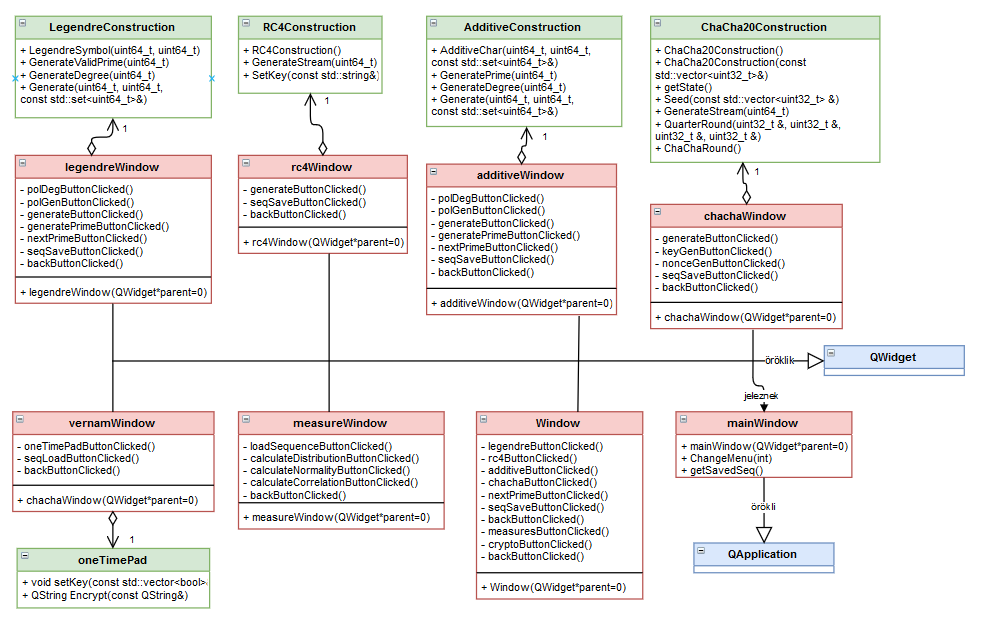
\includegraphics[width=\textwidth]{UML.png}
	\end{minipage}
	\caption{Osztálydiagram}
\end{figure}
\subsubsection*{LegendreConstruction}
Ez az osztály valósítja meg a Legendre konstrukció megvalósítását.

\textbf{\textit{Implementációs döntések}}

A fenti definícióból, a $\left({\frac{a}{p}}\right)$ Legendre-szimbólum értéke akkor 1, ha $a$ kvadratikus maradék modulo $p$, vagyis $\exists k \in \mathbb{Z}$, hogy $a \equiv k^2\ (\textrm{mod}\ p)$ (feltéve, hogy $a$ nem kongruens 0-val $\textrm{mod}\ p$). Ezt ellenőrizni brute-force módszerrel költséges, ezért egy gazdaságosabb számítás kell.

A gazdaságosabb számítás a Legendre-szimbólum tulajdonságait használja ki és rekurzív függvénnyel határozzuk meg az eredményt (ez a függvény később LegendreSymbol néven szerepel). A rekurzió akkor áll meg, ha $a$ 0 vagy 1, ha $a = 0$, akkor $\left({\frac{a}{p}}\right) = 0$, ha $a=1$, akkor $\left({\frac{a}{p}}\right) = 1$. Ha $a \not\in \{0,1\}$, akkor következőképpen állítjuk elő a következő rekurziós lépést:

\begin{enumerate}
	\item Megnézzük, hogy $a$ páros-e, ezt gyorsan meghatározhatjuk, hogy $a$-nak a bitenkénti és műveletét vizsgáljuk az $1$-et reprezentáló bitsorozattal. Ebből következik, hogyha $a$ \& $1 = 0$, akkor $a$ páros, és ekkor a következő redukciót használjuk:
	\begin{enumerate}
		\item  Általánosan igaz, hogy $\left({\frac{ab}{p}}\right) = \left({\frac{a}{p}}\right)\left({\frac{b}{p}}\right)$ (a Legendre-szimbólum a felső változójában teljesen multiplikatív függvény). Mivel $a$ jelen esetben páros, ezért $\left({\frac{a}{p}}\right) = \left({\frac{a/2}{p}}\right)\left({\frac{2}{p}}\right)$. Rekurzív lépésként kiszámoljuk az $\left({\frac{a/2}{p}}\right)$ értékét.
		\item Ki kell még utólag számolni $\left({\frac{2}{p}}\right)$-t. Erre használható a $\left({\frac{2}{p}}\right) = (-1)^{\frac{p^2-1}{8}}$ formula (itt felhasználjuk, hogy a Legendre konstrukciónál $p > 2$, vagyis $p$ páratlan). Mivel $p$ páratlan, ezért könnyen ellenőrizhető, hogy $p^2-1$ mindenképpen osztható lesz 8-cal, így elég annyit ellenőrizni megint, hogy a 8-cal vett kvóciens páros, vagy páratlan. Ezt megint bitenkénti és művelettel ellenőrizzük, ha $p^2-1$ \& $8 \not= 0$ (ahol az \& a bitenkénti és művelet), akkor a $\frac{p^2-1}{8}$ páratlan szám, tehát $\left({\frac{2}{p}}\right) = -1$, egyéb esetben 1.
	\end{enumerate}
	\item Ha $a$ páratlan, akkor:
	\begin{enumerate}
		\item A redukciós formula a következő (kihasználva, hogy $a$ és $p$ relatív prímek): $\left({\frac{a}{p}}\right) = \left({\frac{p}{a}}\right) (-1)^{\frac{p-1}{2}\cdot\frac{a-1}{2}}$. Ez a redukció a kvadratikus reciprocitás tételeként ismert. A rekurziós lépésként ki kell számolni $\left({\frac{p}{a}}\right)$-t itt már egyből $p$-nek az $a$-val vett osztási maradékát adjuk meg a rekurzív hívásba.
		\item Utólag ki kell számolni $(-1)^{\frac{p-1}{2}\frac{a-1}{2}}$-t. Ez nyilvánvalóan akkor lesz $-1$, ha $\frac{p-1}{2}\frac{a-1}{2} = \frac{(p-1)(a-1)}{4}$ páratlan. Mivel $a$ és $p$ is páratlanok, ezért mindenképpen igaz, hogy ez a számláló osztható 4-el, így megint elég csak a 4-el vett kvócienst megnézni, tehát ha $(p-1)(a-1)$ \& $4 \not=0$, akkor a fenti kifejezés $-1$, egyébként 1.
	\end{enumerate}
\end{enumerate}
\textbf{\textit{Metódusok}}

Most minden metódus public és a megadott paraméterek helyessége feltételezhető.

\textit{LegendreConstruction()}

Alapértelmezett default konstruktora van az osztálynak, mivel igazából nincsenek adattagok, csak egy konstans (ez azt adja meg, hogy hány próbát végezzünk a prímkereső algoritmussal), melyet jelenleg nem lehet módosítani.

\textit{int LegendreSymbol(const uint64\_t a, const uint64\_t p)}

Kiszámolja az $\left({\frac{a}{p}}\right)$ Legendre szimbólum értékét.

\textit{uint64\_t GenerateValidPrime(uint64\_t p)}

Olyan prímszám generálása, mely nagyobb egyenlő mint p és a 2 primitív gyöke.

\textit{uint64\_t GenerateDegree(const uint64\_t p)}

Polinom fokszám generálása a $[2, 5\cdot p^\frac{1}{10}]$ intervallumban.

\textit{std::vector$<$bool$>$ Generate(const uint64\_t stream\_size, const uint64\_t p, const std::set$<$uint64\_t$>$\& poly)}

A Legendre konstrukció szerint \textit{stream\_size} méretű bitsorozat generálása és visszaadása \textit{p} prímmel és \textit{poly} polinommal.

\textbf{\textit{Használt globális függvények: }}\textit{GenerateRandomSeed, ModPolynomValue, MillerRabinTest, IsPrimitiveRootOfPrime}

\subsubsection*{RC4Construction}
Ez az osztály az RC4 konstrukció megvalósítása.

\textbf{\textit{Implementációs döntések}}

Ennek a generátornak az implementálása kifejezetten egyszerű , nincs sok buktató dolog és a számolás is gyors, így itt nem kellett semmilyen trükköt bevetni. Az egyet dolog ami megoldásra szorult az outputként kapott számok bitsorozattá konvertálása, de ez is egyszerűen megoldható std::bitset-tel történő konverzióval.

\textbf{\textit{Metódusok}}

\textit{RC4Construction()}

Public metódus, de semmi érdemlegeset nem csinál, a kulcsot később módosítjuk a programban.

\textit{void SetKey(const std::string\& s)}

Public metódus, beállítja a RC4 generáláshoz használt kulcs-stringet.

\textit{std::vector$<$bool$>$ GenerateStream(const uint64\_t stream\_size)}

Public metódus, \textit{stream\_size} méretű stream generálása az RC4 algoritmussal.

\textit{void Init()}

Private metódus, az $S$ tömböt inicializálja az algoritmus leírása szerint.

\textit{void Shuffle()}

Private metódus, az $S$ tömb megkeverése az algoritmus leírása szerint.

\subsubsection*{AdditiveConstruction}
Ez az osztály az additív karakteres konstrukció megvalósítása.

\textbf{\textit{Implementációs döntések}}

Ennek a konstrukciónak az implementálása egyszerű, mely szempont is volt a tervezésekor. Nem ütköztem az implementáció során problémákba, így nem kellett döntéseket hozni.

\textbf{\textit{Metódusok}}

Most minden metódus public és a megadott paraméterek helyessége feltételezhető.

\textit{AdditiveConstruction()}

Default konstruktor, nem inicializálunk semmit egyebet.

\textit{bool AdditiveChar(const uint64\_t n, const uint64\_t p, const std::set$<$uint64\_t$>$\& poly)}

Visszaadja a konstrukció szerinti értéket \textit{p} prímmel és \textit{poly} polinommal az \textit{n}. pozícióban.

\textit{uint64\_t GeneratePrime(uint64\_t p)}

A konstrukciónak megfelelő prímszám generálása mely nagyobb egyenlő mint \textit{p}.

\textit{uint64\_t GenerateDegree(const uint64\_t p)}

Polinom fokszám generálása a $[2, 5\cdot p^\frac{1}{10}]$ intervallumban.

\textit{std::vector$<$bool$>$ Generate(const uint64\_t stream\_size, const uint64\_t p, const std::set$<$uint64\_t$>$\& poly)}

A konstrukció szerinti \textit{stream\_size} hosszúságú bitsorozat generálása \textit{p} prím és \textit{poly} polinom paraméterekkel.

\textbf{\textit{Használt globális függvények: }}\textit{GenerateRandomSeed, ModPolynomValue, MillerRabinTest}

\subsubsection*{ChaCha20Construction}
Ez az osztály a ChaCha20 konstrukció megvalósítása.

\textbf{\textit{Implementációs döntések}}

A ChaCha20 állapota 16 darab 32 bites szóból áll. A reprezentáció kérdéses volt, de úgy döntöttem, hogy a fixen 32 bites uint32\_t típussal felpopulált 16 méretű tömb megfelelő.

Az algoritmus negyedköreinek futtatásánál szükséges a ciklikus shiftelés megvalósítása a 32 bites szavakon. C++-ban erre nincs beépített eszköz, csak sima shiftelésre, de mivel tudjuk, hogy minden szó 32 bites, ezért egy trükkel megvalósítható a ciklikus változat is. Ha van egy $b$ 32 bites szavunk és $n$-el szeretnénk ciklikusan balra shiftelni, akkor a következő kódrészletben vett kifejezésnek pontosan a $b$ $n$-el vett ciklikus balra shiftelése az eredménye (C++ stílusú pszeudokódként): $(b << n) | (b >> (32-n));$. Mivel a túlcsorduló biteket elvesztjük és így a shiftelés irányától függően a megfelelő helyi értékeken 0-ák szerepelnek (ahova ciklikusan át kéne kerülnie a túlcsorduló elemeknek). Így ha bitenként vagyot alkalmazunk a két bitsorozatra, akkor a 0-ás helyi értékek helyén pontosan a túlcsordult részlet lesz.

Az állapot konstans részét bele lehetne égetni az állapottömbbe, de a felhasználói felület oldalon ellenőrzött adatbevitellel dolgozunk, így nem fordulhat elő, hogy hibás állapotot kapjunk. Emiatt itt nincs ellenőrzés az állapot helyességével kapcsolatban. Új állapot megadásánál std::vector-ban adódik át a kívánt érték, ennek első 16 elemét másoljuk be az állapottömbbe.

\textbf{\textit{Metódusok}}

\textit{ChaCha20Construction()}

Default konstruktor, inicializálja az állapot konstans részét, a többit viszont nem, így nem érdemes ezzel nekiállni generálni.

\textit{ChaCha20Construction(const std::vector$<$uint32\_t$>$ \&inbuf)}

Konstruktor, megkapja a kezdeti állapotot az \textit{inbuf} vectorban.

\textit{void Seed(const std::vector$<$uint32\_t$>$ \&inbuf)}

Public metódus, az \textit{inbuf}-ból kimásolja az első 16 elemet az állapotba.

\textit{std::vector$<$bool$>$ GenerateStream(uint64\_t length)}

Public metódus, a ChaCha20 konstrukció szerint a jelenlegi állapottal \textit{length} hosszúságú bitsorozat generálása.

\textit{void QuarterRound(uint32\_t \&a, uint32\_t \&b, uint32\_t \&c, uint32\_t \&d)}

Private metódus, a ChaCha20 negyedkör megvalósítása. Referenciaként adódnak át az értékek, így függvény után az \textit{a}, \textit{b}, \textit{c}, \textit{d} változók már a megváltoztatott állapotot tartalmazzák.

\textit{std::array$<$uint32\_t, 16$>$ ChaChaRound()}

Private metódus, a teljes ChaCha20 kör megvalósítása.

\subsubsection*{oneTimePad}
Ez az osztály a one-time pad titkosítást valósítja meg.

\textit{\textbf{Implementációs döntések}}

A megfelelő karakterek reprezentáláshoz nem volt elég a klasszikus C++ string, mivel az ANSI kódolásban jeleníti meg a karaktereket. Unicode kódolású stringekkel lenne jobb dolgozni és a QT-ben található QString osztály pontosan egy ilyen string típust valósít meg. Emiatt ez az osztály kihasználja a QString ezen tulajdonságát.

Ez az osztály implementálja a szótárat is melyben tároljuk a karakterkódolást. Olyan adatszerkezet lenne jó, mely kétoldalú lekérdezést valósít meg konstans időben, de egy ilyen implementálása dupla letárolás nélkül nem túl egyszerű. Dupla letárolással azonban nagyon könnyű a megoldás, két hashtáblát populálunk fel a megfelelő karakterek-bitsorozat párokkal. Mindegyik hashtábla a C++-os std::unordered\_map típussal valósul meg, mely konstans idejű lekérdezését biztosítja az elemeknek. Az inicializálás a dictionary.txt fájlból történik.

\textit{\textbf{Metódusok}}

\textit{oneTimePad()}

Konstruktor, felépíti a hashtáblákat a dictionary.txt-ből.

\textit{void setKey(const std::vector$<$bool$>$ \&newkey)}

Publikus setter, átállítja a titkosítási kulcsot a \textit{newkey} sorozatára.

\textit{QString Encrypt(const QString \&inputText)}

A titkosítást végző eljárás. Az eredmény és a paraméter is QString-ben tároljuk, hogy a karakterek Unicode-al legyenek továbbra is reprezentálva.
\subsubsection*{mainWindow}
Ez az osztály a grafikus felület fő vezérlését és megjelenítést valósítja meg. Szorosan együttműködik a többi ablak osztállyal az alkalmazás irányításában. A sorozatok lementését is ez az osztály végzi, a savedSeq adattagban lementhetünk egy bitsorozatot amit az alkalmazáson keresztül generáltunk.

Ez az osztály a QMainWindow QT osztálynak gyermekosztálya.

\textit{\textbf{Metódusok}}

A QMainWindow-ból öröklött metódusokról nem értekezem, ennek az osztálynak a funkciói megtalálhatóak a QT dokumentáció részeként. Minden függvény publikus.

\textit{mainWindow(QWidget *parent = 0)}

Az osztály konstruktora. Lefuttatja a QMainWindow konstruktorát a kapott paraméterrel, inicializálja az almenüket és a vezérléshez szükséges eszközöket.

\textit{void ChangeMenu(const int i)}

Megváltoztatja az éppen aktív almenüt az i. indexűre (minden almenü egy indexszel van azonosítva).

\textit{std::vector$<$bool$>$\& getSavedSeq()}

Visszaadja az éppen lementett sorozatot.

\textit{void setSavedSeq(const std::vector$<$bool$>$ \&seq)}

Lementi a paraméterként kapott sorozatot a savedSeq változóba.

\subsubsection*{Window}
Az alapmenüt megvalósító osztály, mely a QWidget gyermeke.

\textit{\textbf{Metódusok}}

A QWidget osztályból örökölt metódusokról nem értekezem, ezek a QT dokumentációba megtalálhatóak.

\textit{Window(QWidget *parent = 0)}

A Window konstruktora, inicializálja az adattagokat és lefuttatja a QWidget konstruktorát a kapott paraméterrel.

\textit{void makeButtons(), void setButtonsSize(), void setButtonsSender()}

Private segédfüggvények, az inicializálás részfeladatait végzik.

\textit{\textbf{Eseménykezelés}}

Az eseménykezelést végző QT object slotoknak a leírása, ezek mind private slotok.

\textit{void legendreButtonClicked(), void rc4ButtonClicked(), void additiveButtonClicked(), void chachaButtonClicked(), void measuresButtonClicked(), void cryptoButtonClicked()}

Az almenük közti váltások gombjaira írt slotok. A gombok megnyomásakor a kért almenüt jeleníti meg a program.

\textit{void quitButtonClicked()}

A kilépés gombja, az alkalmazás futását szabályosan megszünteti.

\subsubsection*{legendreWindow}

A Legendre-konstrukció kezelését megvalósító osztály. A QWidget gyermekosztálya.

\textbf{\textit{Metódusok}}

\textit{legendreWindow(QWidget *parent = 0)}

Konstruktor, lefuttatja a QWidget konstruktorát a kapott paraméterrel és inicializálja a szükséges adattagokat.

\textit{void makeLengthForm(), void makePolDeg(), void makePrimeForm(), void makePolForm(), void makeSequenceForm()}

Az inicializáláshoz használt private segédmetódusok.

\textbf{\textit{Eseménykezelés}}

\textit{void polDegButtonClicked()}

Polinom fokszám generálását kezelő slot. Meghíváskor begyűjti a bemeneti mezőkből a szükséges adatokat és ez alapján generál, az eredmény a polDegLineEdit-be kerül.
Hibákat is kezel, rossz prím bemenet esetén hibajelzést ír ki a grafikus felületre.

\textit{void polGenButtonClicked()}

Polinom generálását kezelő slot. Meghíváskor begyűjti a fokszám és prím adatokat és ez alapján generál megfelelő polinomot, az eredmény a polTextEdit-be kerül. Ha rossz a bemenet, akkor hibajelzést ír ki.

\textit{void generateButtonClicked()}

Sorozatgenerálás eseményét kezelő slot. Meghíváskor begyűjti az összes paramétert a Legendre-konstrukcióhoz és ez alapján generál, az eredmény a seqTextEdit-be kerül. Hiba esetén hibaüzenet kerül kiírásra.

\textit{void generatePrimeButtonClicked()}

Prímszám generálás slotja. Híváskor prímszámot generál mely megfelel a Legendre-konstrukciónak, az eredmény a primeLineEdit-be kerül. Hibás hossz bemenet esetén hibaüzenet kerül kiírásra.

\textit{void nextPrimeButtonClicked()}

Következő prím slotja. Híváskor az első, a jelenleginél nagyobb, prímet állítja elő mely megfelel a Legendre konstrukciónak, az eredmény a primeLineEdit-be kerül. Hibás prím bemenet esetén hibaüzenet kerül kiírásra.

\textit{void seqSaveButtonClicked()}

A jelenlegi sorozat lementésének slotja. A seqTextEdit-ben lévő sorozatot menti le a mainWindow savedSeq-jébe.

\textit{backButtonClicked()}

Visszalépés slotja, visszaadja a vezérlést a főmenünek.

\textbf{\textit{Használt globális függvények: }} \textit{displayError, GenerateSimpleModPoly}

\subsubsection*{rc4Window}

Az RC4 konstrukció kezelését megvalósító osztály. A QWidget gyermekosztálya.

\textit{\textbf{Metódusok}}

\textit{rc4Window(QWidget *parent = 0)}

Konstruktor, lefuttatja a QWidget konstruktorát a kapott paraméterrel és inicializálja az adattagokat.

\textit{void makeLengthForm(), void makeKeyForm(), void makeSequenceForm()}

Az inicializáláshoz használt private segédmetódusok.

\textit{\textbf{Eseménykezelés}}

\textit{void generateButtonClicked()}

Az RC4 konstrukcióval való sorozat generálásának slotja. A generálás a bevitt paraméterek alapján történik és ezután az eredmény a seqTextEdit-be kerül. Hibás bemenet esetén hibaüzenet kerül kiírásra.

\textit{void seqSaveButtonClicked()}

A generált sorozat mentésének slotja. A mainWindow savedSeq-jébe kerül a seqTextEdit tartalma.

\textit{void backButtonClicked()}

Visszalépés slotja, a vezérlés visszaadása a főmenünek.

\textit{\textbf{Használt globális függvények: }}\textit{displayError}

\subsubsection*{additiveWindow}

Az additív karakteres konstrukció kezelését megvalósító osztály. A QWidget gyermekosztálya.

\textbf{\textit{Metódusok}}

\textit{additiveWindow(QWidget *parent = 0)}

Konstruktor, a QWidget konstruktorát lefuttatja a kapott paraméterrel és inicializálja az adattagokat.

\textit{void makeLengthForm(), void makePolDeg(), void makePrimeForm(), void makePolForm(), void makeSequenceForm()}

Inicializáláshoz használt private segédmetódusok.

\textbf{\textit{Eseménykezelés}}

\textit{void polDegButtonClicked()}

Polinom fokszám generálását kezelő slot. Meghíváskor begyűjti a bemeneti mezőkből a szükséges adatokat és ez alapján generál, az eredmény a polDegLineEdit-be kerül.
Hibákat is kezel, rossz prím bemenet esetén hibajelzést ír ki a grafikus felületre.

\textit{void polGenButtonClicked()}

Polinom generálását kezelő slot. Meghíváskor begyűjti a fokszám és prím adatokat és ez alapján generál megfelelő polinomot, az eredmény a polTextEdit-be kerül. Ha rossz a bemenet, akkor hibajelzést ír ki.

\textit{generateButtonClicked()}

Sorozatgenerálás eseményét kezelő slot. Meghíváskor begyűjti az összes szükséges paramétert az Additív konstrukcióhoz és ez alapján generál. Az eredmény a seqTextEdit-be kerül. Hiba esetén hibaüzenet kerül kiírásra.

\textit{generatePrimeButtonClicked()}

Prímszám generálás slotja. Híváskor új prímszámot generál mely megfelel az Additív karakteres konstrukciónak, az eredmény a primeLineEdit-be kerül. Hibás hossz bemenet esetén hibaüzenet kerül kiírásra.

\textit{void nextPrimeButtonClicked()}

Következő prím slotja. Híváskor az első, a jelenleginél nagyobb, prímet állítja elő mely megfelel az Additív karakteres konstrukciónak, az eredmény a primeLineEdit-be kerül. Hibás prím bemenet esetén hibaüzenet kerül kiírásra.

\textit{void seqSaveButtonClicked()}

A generált sorozat mentésének slotja. A mainWindow savedSeq-jébe kerül a seqTextEdit tartalma.

\textit{void backButtonClicked()}

Visszalépés slotja, visszaadja a vezérlést a főmenünek.

\textit{\textbf{Használt globális függvények: }}\textit{displayError, GenerateSimpleModPoly}

\subsubsection*{chachaWindow}

Az ChaCha20 konstrukció kezelését megvalósító osztály. A QWidget gyermekosztálya.

\textit{\textbf{Metódusok}}

\textit{chachaWindow(QWidget *parent = 0)}

Konstruktor, inicializálja az adattagokat és lefuttatja a QWidget osztály konstruktorát a kapott paraméterrel.

\textit{void makeLengthForm(), void makeKeyForm(), void makeCounterForm(), void makeNonceForm(), void makeSequenceForm()}

Az inicializáláshoz használt private segédmetódusok.

\textit{\textbf{Eseménykezelés}}

\textit{void generateButtonClicked()}

Sorozatgenerálás eseményét kezelő slot. Meghíváskor begyűjti az osztály az összes paramétert a ChaCha20 konstrukcióhoz és ez alapján generál. Az eredmény a seqTextEdit-be kerül. Hiba esetén hibaüzenet kerül kiírásra.

\textit{void keyGenButtonClicked()}

Kulcs generálásának slotja. Híváskor a program generál egy véletlenszerű kulcsot (8*32 bitet) a ChaCha20 állapotba, eredmény a keyEdit-be kerül.

\textit{void nonceGenButtonClicked()}

Nonce generálásának slotja. Híváskor a program generál egy véletlenszerű nonce-ot (3*32 bitet) az ChaCha20 állapotba, eredmény a nonceEdit-be kerül.

\textit{void seqSaveButtonClicked()}

A generált sorozat mentésének slotja. A mainWindow savedSeq-jébe kerül a seqTextEdit tartalma.

\textit{void backButtonClicked()}

Visszalépés slotja, visszaadja a vezérlést a főmenünek.

\textit{\textbf{Használt globális függvények: }}\textit{GenerateRandomSeed}

\subsubsection*{measureWindow}

A mértékek kiszámításának kezelését megvalósító osztály. A QWidget gyermekosztálya.

\textit{\textbf{Metódusok}}

\textit{measureWindow(QWidget *parent = 0)}

Konstruktor, inicializálja az adattagokat és lefuttatja a QWidget konstruktorát a kapott paraméterrel.

\textit{void makeSequenceForm(), void makeDistrForm(), void makeNormalityForm(), void makeCorrelationForm()}

Az inicializáláshoz használt private segédmetódusok.

\textit{\textbf{Eseménykezelés}}

\textit{void loadSequenceButtonClicked()}

A jelenleg lementett sorozat betöltésének slotja. Híváskor a mainWindow savedSeq-jében lévő sorozatot betölti a seqTextEdit-be.

\textit{void calculateDistributionButtonClicked()}

A jól-eloszlás mérték számolásának slotja. Híváskor a seqTextEdit-ben lévő sorozatra kiszámolja a jól-eloszlás mértéket és az eredményt a distrLineEdit-be írja.

\textit{void calculateNormalityButtonClicked()}

A normalitás mérték számolásának slotja. Híváskor a seqTextEdit-ben lévő sorozatra kiszámolja a normalitás mértéket és az eredményt a normalityLineEdit-be írja.

\textit{void calculateCorrelationButtonClicked()}

A k-ad rendű korreláció mérték számolásának slotja. Híváskor a seqTextEdit-ben lévő sorozatra közelíti a k-ad rendű korrelációt. A rendet a correlationDegLineEdit-ből, a menetek számát a correlationRoundsLineEdit-ből tölti be. Hibás adat esetén hibaüzenet kerül kiírásra a képernyőre.

\textit{void backButtonClicked()}

Visszalépés slotja, visszaadja a vezérlést a főmenünek.

\textit{\textbf{Használt globális függvények: }}\textit{wellDistributionMeasure, normalityMeasure, kCorrelationApprox, displayError}

\subsubsection*{vernamWindow}

A one-time pad titkosítás kezelését megvalósító osztály. A QWidget gyermekosztálya.

\textbf{\textit{Metódusok}}

\textit{vernamWindow(QWidget *parent = 0)}

Konstruktor, inicializálja az adattagokat és a QWidget konstruktorát lefuttatja a kapott paraméterrel.

\textit{void makeTextForm(), void makeBitSeqForm(),	void makeResultForm()}

Az inicializáláshoz használt private segédmetódusok.

\textbf{\textit{Eseménykezelés}}

\textit{void oneTimePadButtonClicked()}

A titkosítás futtatásának slotja. Híváskor az inputTextEdit-ből és a  seqTextEdit-ből tölti be az adatokat a titkosításhoz. A titkosítás eredménye a resultTextEdit-be kerül. Hibás bemenet esetén hibaüzenet kerül kiírásra a képernyőre.

\textit{void seqLoadButtonClicked()}

A sorozat betöltésének slotja. Híváskor a mainWindow savedSeq-jében lementett sorozatot betölti a seqTextEdit-be.

\textit{void backButtonClicked()}

Visszalépés slotja, visszaadja a vezérlést a főmenünek.

\textit{\textbf{Használt globális függvények: }}\textit{displayError}

\subsubsection{Globális függvények}
Az osztály nélkül definiált globális függvények több fejállományra bontva szerepelnek a kódban. Ezeknek dokumentáció a fejállományok szerint fog történni.

\subsubsection*{ModArithmeric}
Moduláris számításokkal kapcsolatos műveleteket tartalmaz.

\textit{\textbf{Függvények}}

\textit{uint64\_t ModMul(uint64\_t a, uint64\_t b, const uint64\_t mod)}

Ez a függvény \textit{a}*\textit{b}-t számolja ki a \textit{mod} 
maradékosztályban.

\textit{uint64\_t ModPow(uint64\_t base, uint64\_t exp, const uint64\_t mod)}

Gyors moduláris hatványozás, $\textit{base}^\textit{exp}$ kiszámolására, \textit{mod} maradékosztályban. Használja a ModMul függvényt.

\textit{uint64\_t Pow(uint64\_t base, uint64\_t exp)}

Gyors hatványozás moduloosztály nélkül.

\textit{uint64\_t ModSub(uint64\_t a, uint64\_t b, const uint64\_t mod)}

Moduláris kivonás, $\textit{a}-\textit{b}$-t számolja ki \textit{mod} maradékosztályban.

\textit{std::set$<$uint64\_t$>$ GenerateSimpleModPoly(const uint64\_t modulus, const unsigned int degree)}

Csakis egyszeres gyökökkel rendelkező polinom generálása \textit{modulus} maradékosztályban, \textit{degree} fokszámmal. Használja a GenerateRandomSeed() függvényt.

\textit{uint64\_t ModPolynomValue(const std::set$<$uint64\_t$>$ \&poly, const uint64\_t mod, uint64\_t var)}

Polinom helyettesítési értékének kiszámolása \textit{var} helyen és \textit{mod} maradékosztályban. Használja a ModMul és a ModSub függvényeket.

\textit{std::vector$<$uint64\_t$>$ GetPrimeFactors(uint64\_t n)}

Megkeresi az \textit{n} szám összes valós osztóját és ezeket egy std::vector-ba helyezve adja vissza (minden osztó csak egyszer szerepel benne).

\subsubsection*{PrimeArithmetic}

Prímtesztet, prímekhez kapcsolható számításokat tartalmaz.

\textit{\textbf{Függvények}}

\textit{bool IsPrimitiveRootOfPrime(const uint64\_t n, const uint64\_t p)}

Kiszámolja, hogy \textit{n} primitív gyök-e \textit{p} maradékosztályban, ahol \textit{p} prím. Az algoritmus az alapján működik, hogy a primitív gyök tulajdonság ekvivalens azzal, hogy \textit{n} rendje \textit{p}$-1$-el a maradékosztályban, mivel prím a második paraméter, és a \textit{p}$-1$ osztóit kell megkeresni, ha minden $d$ osztóra $n^\frac{\textit{p}-1}{d} \not\equiv 1 (\textrm{mod}\ p)$, akkor n primitív gyök. Használja a GetPrimeFactors függvényt.

\textit{bool MillerRabinTest(const uint64\_t n, const int k)}

Miller-Rabin valószínűségi prímteszt végrehajtása \textit{k} darab menettel \textit{n}-en. Kis prímekre mindenképpen tesztel, de utána \textit{k} darab véletlen számmal próbálkozik. Ha átmegy az összes teszten, akkor lesz igaz az eredmény. Használja a GenerateRandomSeed() függvényt.

\subsubsection*{SeedGenerator}

Ez csak egy függvényt tartalmazó fejállomány, az adott számítógép működéséből készít entrópiát az egyszerűbb véletlenségi feladatokhoz, ahol elég az, hogy kapjunk egyenletesen eloszláson számokat.

\textit{\textbf{Függvények}}

\textit{static void SeedFunction()}

Statikus függvény amit csak azért hozunk létre, hogy a memóriacímét lekérdezzük, ezáltal is növelve az entrópia mértékét.

\textit{std::seed\_seq GenerateRandomSeed()}

Több forrásból felépíti a seed sorozatunkat. Az entrópiát a gépi időből, memóriakezelésből és szálkezelésből szerzi. Összes módszer pontosan: idő, statikus változó (számláló) értéke és címe, lokális változó címe, dinamikusan foglalt változó címe, a SeedFunction() címe, a C++ \_Exit() függvényének címe. Egy generálás után mindig növeljük a számláló értékét.

\subsubsection*{Measurements}
A mértékek kiszámolását végző függvények ebben a fejállományban helyezkednek el. Jelen esetben a 3 implementált mértékről külön értekezem.

\textit{\textbf{Jól-eloszlás}}

A jól-eloszlás mérték kiszámolása a legegyszerűbb a 3 közül, itt is fontos volt azonban, hogy a megvalósításnál a matematikai definíciót ne pazarlóan valósítsuk meg. A jól-eloszlás ugyebár valamilyen $a$ kezdőpozíciótól számolja a $b$ eltolással vett indexeken lévő bitek összegét minden lehetséges $M$ végpozícióig (bővebben ld. a Mértékek fejezetet).

Itt igazából végpozícióval lehet úgy tenni, mintha nem létezne mint ciklusváltozó, az maximum keresését egybe lehet futtatni a bitek összegzésével. Tehát csak a lehetséges kezdőpozíciók és eltolások szerint keresünk maximumot, és az összegek között számolás közben frissítjük a maximális összeget. 

Ezzel az optimalizálással megvalósított függvény a következő: \textit{uint64\_t wellDistributionMeasure(const std::vector$<$bool$>$ \&seq)}. Ez a fenti módon határozza meg a seq-ben lévő sorozat jól-eloszlás mértékét.

Létezik a kezdetleges implementációból egy függvény mely a definícióban szereplő $U(E_N, M, a, b)$ függvényt valósítja meg: \textit{int64\_t UMeasure(const std::vector$<$bool$>$ \&seq, const uint32\_t sum\_length, const uint32\_t start\_pos, const uint32\_t step)}.

\textit{\textbf{Normalitás}}

A normalitás mértéknél a legnagyobb kihívást az összes vizsgálandó részsorozat effektív legenerálása jelentette. Leegyszerűsítve arra kellett algoritmust írni, mely az összes max. $k \in \mathbb{N}$ hosszúságú bitsorozatot előállítja (kivéve a 0 hosszút). Erre egy $(k+1)^2$ méretű mátrixot használunk, hogy a prefixek letárolásával tudjuk előállítani mindig a következő részsorozatokat. Így a mátrixba megtalálható az összes vizsgálandó sorozat, és a generálás gyors. 0 hosszúságú sorozatról kezdünk, és minden lépésben a már meglévő prefixekhez fűzünk hozzá 0-kat és 1-eseket és ezeket behelyezzük a mátrixba. Az eljárás végén a mátrix megfelelő indexein az összes részsorozat megtalálható. Így viszont nincs különszedve a k-ad rendű normalitások számolása.

A másik költséges dolog az volt, hogy hogyan keressük meg a részsorozatok előfordulásának számát. Bár itt bitekről van szó és vannak bitsorozatokra jobb matchelő algoritmusok melyek kihasználják, hogy nem csak egyesével tudunk biteket címezni. Ezt azonban a jelenlegi reprezentációval nem lehet megtenni, az vector<bool>-ban nem tudunk több bitre egyszerre hivatkozni. Emiatt inkább string-matchelésre vezetett vissza a probléma, ezért a Rabin-Karp algoritmust implementáltam a bitsorozatos reprezentációra.

A fenti optimalizálásokkal a számolást a következő függvény valósítja meg: \textit{long double normalityMeasure(const std::vector$<$bool$>$ \&seq)}.

A definíció szerinti $T(E_N), M, X)$ függvényt, illetve a k-ad normalitást is implementáltam, ezeket sorban a \textit{uint64\_t TMeasure(const std::vector$<$bool$>$ \&seq, const uint32\_t max\_pos, const std::vector$<$bool$>$ \&subSeq)}, illetve a \textit{long double kNormality(std::vector$<$bool$>$ \&seq, const uint32\_t k)} függvények valósítják meg.

\textit{\textbf{Korreláció}}

Ez a számítás a legköltségesebb a három mérték közül. A fő költséget a sorozat mérete alapján generálandó sorozatok száma. Az összes eltolássorozat számossága $N$ méretű sorozat és $k$-ad rendű korreláció esetén $\binom{N}{k}$. A teljes algoritmus költsége még ennél is több számítást igényel, a teljes korreláció esetén $k \leq log_2(N)$, így ezek a binomiális együtthatók már pl. $N=1000$-re is nagyon nagyok. 

A k-ad rendű korreláció pontos számolásra a jelenleg legjobban teljesítő megoldás egy rekurzív algoritmus lett. Az összes kellő eltolássorozat legenerálása így a leggyorsabb. Próbálkoztam iteratív módon is leprogramozni a számítást, de a teljesítmény picivel rosszabb volt a rekurzívnál. Az iteratív módszereknél az is nehéz feladat, hogy a sorozatokat hogyan soroljuk fel. A rekurzív megoldás egy tömbbe tárolja a felsorolandó sorozatokat, mely ha egy k hosszú sorozat lesz a rekurzióban, akkor vizsgáljuk meg. Ezt a megoldást a \textit{uint64\_t kCorrelation(const std::vector$<$bool$>$ \&seq, const uint32\_t k)} valósítja meg, mely a \textit{seq}-ben kapott sorozatra számolja ki a \textit{k}-ad rendű korreláció mértéket.

Mivel ezen mérték számolása ilyen hosszú már kisebb sorozatokra is, ezért a jelenlegi programban egy közelítő megoldást implementáltam. Véletlen kiválasztott sorozatok között keresünk csak maximumot, ezzel alsó becslést tudunk adni a k-ad rendű és ezzel egyben a teljes korrelációra. Ezt a megoldást a \textit{uint64\_t kCorrelationApprox(const std::vector$<$bool$>$ \&seq, const uint32\_t k, const uint32\_t rounds)} függvény valósítja meg, a \textit{seq}-benk apott sorozatra \textit{rounds} darab véletlen kiválasztott \textit{k} hosszúságú sorozatra kiszámolva a definícióban szereplő $V(E_N, M, D)$ mennyiséget minden megfelelő $M$ kezdőpozícióval.
\subsection{Tesztelés}
Az eddig tárgyalt programrészletek tesztelésére létrehoztam egy tesztelő környezetet a Catch keretrendszer használatával. Ebben a fejezetben felsorolom az elvégzett tesztelést. A program mindegyik tárgyalt tesztesetnek megfelelt. A tesztelő megtalálható a Testing mappában.

A teszteseteket próbáltam úgy elkészíteni, hogy elég általánosak legyenek és minél több működést fedjenek le.
\subsubsection*{Tesztesetek}
\begin{enumerate}
	\item \bfseries Miller-Rabin prímteszt:
	\normalfont Mindegyik esetben 40 próbával futtatjuk a tesztet. Vizsgált esetek és várt eredmény:
	\begin{enumerate}
		\item Pozitív: 13, 1619, 10120459
		\item Negatív: 1561, 15847, 274613
	\end{enumerate}
	\item \bfseries Prím faktorizáció:
	\normalfont Prímosztók megkeresése. Az osztók mennyiségére és megfelelő értékére is ellenőriz. Vizsgált esetek és várt eredmény:
	\begin{enumerate}
		\item 13: 13
		\item 84: 2, 3, 7
		\item 35147: 7, 5021
		\item: 7140133: 7, 11, 13, 1019
	\end{enumerate}
	\item \bfseries Primitív gyök eldöntése:
	\normalfont Prímszám modulo osztályában eldönti, hogy egy szám primitív gyök-e. Vizsgált esetek és várt eredmény:
	\begin{enumerate}
		\item Pozitív - (Szám: 3, Prím: 7), (Szám: 10, Prím: 97)
		\item Negatív - (Szám: 7, Prím: 157), (Szám: 2, Prím: 199)
	\end{enumerate}
	\item  \bfseries Moduláris szorzás:
	\normalfont $m$ maradékosztályban, $a\cdot b$ számolása. Vizsgált esetek és várt eredmény:
	\begin{enumerate}
		\item $a=6, b = 9, m = 7$, $a \cdot b = 5$
		\item $a=2, b = 99, m=101$, $a \cdot b = 97$
		\item $a=28902, b=467, m=13$, $a \cdot b = 10$
	\end{enumerate}
	\item  \bfseries Moduláris hatványozás:
	\normalfont $m$ maradékosztályban, $a^b$ számolása. Vizsgált esetek és várt eredmény:
	\begin{enumerate}
		\item  $a = 4, b = 7, m = 15$, $a^b=4$
		\item  $a = 3, b = 13, m = 23$, $a^b=9$
		\item  $a = 9, b = 156, m = 7$, $a^b=1$
	\end{enumerate}
	\item \bfseries Moduláris kivonás:
	\normalfont $m$ maradékosztályban, $a-b$ számolása. Vizsgált esetek és várt eredmény:
	\begin{enumerate}
		\item  $a = 5, b = 4, m = 7$, $a-b=1$
		\item  $a = 3, b = 1, m = 101$, $a-b=2$
		\item  $a = 3, b = 5, m = 101$, $a-b=99$
		\item $a = 10, b = 3, m = 5$, $a-b=2$
		\item  $a = 2, b = 9, m = 11$, $a-b=4$
		\item $a=138, b=217, m=13$, $a-b=12$
	\end{enumerate}
	\item \bfseries Moduláris polinom helyettesítési értéke:
	\normalfont $m$ maradékosztályban $f \in Z_m[x]$, $x \in Z_m$ helyen. Vizsgált esetek és várt eredmények:
	\begin{enumerate}
		\item $f(x)=(x-5)(x-7)(x-10)$:
		\\ $m=13$, $x=5$, $f(x) = 0$ 
		\\ $m=13$, $x=2$, $f(x) = 10$
		\\ $m=101$, $x=39$, $f(x) = 40$
		\item $f(x)=(x-1)(x-5), m = 101, x = 3, f(x) = 97$
	\end{enumerate}
	\item \bfseries Legendre-szimbólum:
	\normalfont A $\left({\frac{a}{p}}\right)$ számolásának tesztje. Vizsgált esetek és várt eredmények:
	\begin{enumerate}
		\item $a = 28, p = 7$, $\left({\frac{a}{p}}\right) = 0$
		\item $a = 30, p = 127$, $\left({\frac{a}{p}}\right) = 1$
		\item $a = 483600, p = 61$, $\left({\frac{a}{p}}\right) = -1$
		\item $a = 12345, p = 331$, $\left({\frac{a}{p}}\right) = -1$
	\end{enumerate}
	\item \bfseries Legendre prím generálás:
	\normalfont Az első Legendre-konstrukcióhoz megfelelő $p$ prímszám generálása, mely nagyobb egyenlő mint $n$. Vizsgált esetek és eredmények:
	\begin{enumerate}
		\item $n = 100$, $p = 101$
		\item $n = 200$, $p = 211$
		\item $n = 20000$, $p = 20029$
	\end{enumerate}
	\item  \bfseries Legendre-sorozat generálás teszt:
	\normalfont Legendre-konstrukció szerinti generálás, 10 hosszú sorozat, $p = 101$, $f \in Z_p[x], f(x) = (x-1)(x-5)$, várt eredmény:	$1101011010$.
	\item \bfseries RC4-sorozat generálás teszt:
	\normalfont RC4 szerinti generálás, 10 hosszú sorozat, kulcs értéke (idézőjelek nélkül): "This is a good key". Várt eredmény: $0001111100$
	\item \bfseries Additív karakteres-sorozat generálás teszt:
	\normalfont Additív karakteres generálás, 10 hosszú sorozat, $p = 23$, $f \in Z_p[x], f(x) = (x-1)(x-5)$. Várt eredmény: 1100011001
	\item \bfseries ChaCha20 tesztje:
	\normalfont  A ChaCha20 negyedkört és a teljes kört az IRTF által publikált RFC 8439-ben specifikált teszt vektorok szerint teszteltem.
	\\ A stream generálás egy tesztjét még elvégeztem:
	Input állapot (hexadecimális alakban): \\
	    61707865, 3320646e, 79622d32, 6b206574, \\
		03020100, 07060504, 0b0a0908, 0f0e0d0c, \\
		13121110, 17161514, 1b1a1918, 1f1e1d1c, \\
		00000001, 09000000, 4a000000, 00000000 \\
	10 hosszú sorozat generálása, várt eredmény: $1110010011$
	\item \bfseries Mértékek tesztje:
	\normalfont Példasorozat: $111001011$, mértékek várt eredményei:
	\begin{enumerate}
		\item Jól-eloszlás: $3$
		\item Normalitás: $1.5$
		\item 3-ad rendű korreláció: 6
	\end{enumerate}
\item \bfseries One-time Pad titkosítás:
\normalfont Titkosítandó sorozat: $1010110$, kulcs: $0110010$. Várt eredmény: $1100100$
\end{enumerate}
\subsection{Fejlesztési lehetőségek}
A program még továbbfejleszthető több módon is. A legkézenfekvőbb újabb generátor konstrukciók implementálása és vizsgálata a mértékekkel, ez a felhasználói oldalról sokat jelent. Lehetséges megvalósítani újabb mértékeket is, pl. szimmetria mértéket \cite{symmetry}. 

Grafikonok megjelenítése és statisztikák számolásának implementálása a számolt mértékekből. Ezekkel tovább lehet elemezni a megvalósított konstrukciókat.
\section{Összefoglaló}
A dolgozatban kitértem mind a matematikai, mind az ipari alkalmazások szempontjából készített pszeudovéletlen generátorokra. Megvalósított és bemutatott konstrukciók voltak a Legendre-szimbólumos, RC4, additív karakteres és ChaCha20 konstrukciók. A megvalósított generátoroknak a vizsgálatára és alkalmazására is kitértem, a statisztikai mértékekkel illetve a One-time pad titkosítással.

A programmal tett vizsgálataim során azt tapasztaltam, hogy a Legendre és additív karakteres konstrukció az eddig belátott tulajdonságok szerint (lásd:  \cite{additive} és \cite{largefam}) jó eredményeket ad a megvalósított mértékekkel.

Saját vizsgálataim alapján az RC4 konstrukciónál a mértékek eredménye nagyobb szórású mint a többi generátornak. A kulcsoktól függően az eredmények kiugróan nagyok és alacsonyak is voltak, ez lehet további vizsgálódás tárgya.

A ChaCha20 konstrukció jól teljesített a mértékekkel, átlagosan jó eredmények születtek. Ez alátámasztja azt, hogy az eddigi vizsgálatok alapján (lásd: \cite{salsaattack} és \cite{salsadiffcrypt}) a Salsa/ChaCha család elég jó tulajdonságokkal rendelkező generátorcsoport.
\section{Irodalomjegyzék}
	\renewcommand\refname{}
\begin{thebibliography}{3}
	\bibitem{shannon}
	Shannon, C.E.: \textit{Communication Theory of Secrecy Systems}, Bell System Technical Journal, 28 (4), 1949, [656–715].
	\bibitem{borel}
	E. Borel: \textit{Leçons sur la théorie des fonctions}, 2nd ed. (1914), [850-864].
	\bibitem{knuth}
	D. E. Knuth: \textit{A számítógép-programozás művészete}, Műszaki Könyvkiadó, Budapest, 1994.
	\bibitem{kolmogorov}
	A. Kolmogorov: \textit{Three Approaches to the Quantitative Definition of Information}, Problemy Peredachi Informatsii 1, 1965, [3-11].
	\bibitem{sarkozymauduit}
	C.Mauduit, A.Sárközy: \textit{On finite pseudorandom binary sequences I:The measures of pseudorandomness, the Legendre symbol}, Acta Arith, 82, 1997, 365-377.
	\bibitem{rcleak}
	"Thank you Bob Anderson", Cypherpunks (levelezői lista), 1994, Archiválva: \url{http://cypherpunks.venona.com/date/1994/09/msg00304.html}, 2019.04.29.
	\bibitem{additive}
	C.Mauduit, J.Rivat, A.Sárközy: \textit{Construction of pseudorandom binary sequences using additive characters}, Monatshefte Math, 141, 2004, [197-208].
	\bibitem{salsa}
	Daniel J. Bernstein: \textit{The Salsa20 family of stream ciphers}, \url{https://cr.yp.to/snuffle/salsafamily-20071225.pdf}, 2019.04.29.
	\bibitem{chacha}
	Daniel J. Bernstein: \textit{The ChaCha family of stream ciphers}, \url{https://cr.yp.to/chacha.html}, 2019.04.29.
	\bibitem{RFC}
	Y. Nir, Dell EMC, A. Langley, Google, Inc.: \textit{ChaCha20 and Poly1305 for IETF Protocols}, RFC, 8439, 2018, \url{https://tools.ietf.org/html/rfc8439}, 2019.04.29.
	\bibitem{salsaattack}
	Zhenqing Shi, Bin Zhang, Dengguo Feng, Wenling Wu: \textit{Improved Key Recovery Attacks on Reduced-Round Salsa20 and ChaCha. ICISC'12 Proceedings of the 15th International Conference on Information Security and Cryptology}, Lecture Notes in Computer Science, 7839, 2012, [337–351], ISBN-978-3-642-37681-8
	\bibitem{salsadiffcrypt}
	Nicky Mouha, Bart Preneel: \textit{Towards Finding Optimal Differential Characteristics for ARX: Application to Salsa20}, 2013,  \url{https://eprint.iacr.org/2013/328.pdf}, 2019.04.29.
	\bibitem{cvalue}
	N. Alon, Y. Kohayakawa, C. Mauduit, C. G. Moreira, V. Rödl: \textit{Measures of pseudorandomness for finite sequences: minimal values}, Combin. Prob. Comput., 15, 2005, [1-29]
	\bibitem{symmetry}
	Katalin Gyarmati: \textit{On a pseudorandom property of binary sequences}, The Ramanujan Journal, 8, 2004, [289-302]
	\bibitem{largefam}
	L. Goubin, C. Mauduit, A. Sárközy: \textit{Construction of large families of pseudorandom binary sequences}, J. Number Theory, 106, 2004, [56-59]
\end{thebibliography}
\end{document}